% $Id$
%

\documentclass{scrbook}
%\documentclass[black,pi]{texdiplom}
\usepackage{pslatex}
\usepackage{varioref}
\usepackage{tabularx}
\usepackage{graphicx}
\usepackage{caption}
\usepackage{subcaption}
\usepackage{url}
\usepackage{fancyhdr}
\usepackage{xspace}
\usepackage{booktabs}
\usepackage{hyperref}
\usepackage{textcomp}
\usepackage{hyphsubst} % trennung

\usepackage{afterpage}

% remove from final version
%\usepackage[all,light]{draftcopy}

%\usepackage[Sonny]{fncychap}
%\usepackage{moreverb}
\usepackage{listings}
\usepackage{ifpdf}
\usepackage{float}

\renewcommand{\sfdefault}{psx}
\renewcommand{\rmdefault}{psx}
%\renewcommand{\ttdefault}{pcr}

\newcommand{\node}[1]{\texttt{#1}}


% no more than 2 floats per page
%\setcounter{totalnumber}{2}

% allow [H]
%\restylefloat{figure}

\lstset{basicstyle=\ttfamily \footnotesize,
        showstringspaces=false,
        float=tbp,
        captionpos=b,
        frame=single,
        escapechar=\%,
        language={}}


\makeatother
\sloppy

\ifpdf
  \DeclareGraphicsExtensions{.pdf,.png}
\else
  \DeclareGraphicsExtensions{.eps,.ps}
\fi 

\title{MGX User Guide}
\author{Sebastian Jaenicke\\sjaenick@CeBiTec.Uni-Bielefeld.DE}

\begin{document}
\frontmatter
\maketitle
\cleardoublepage

\newpage
\thispagestyle{empty}

\tableofcontents

\mainmatter


\chapter{Installation}
\label{installation}

\section{Prerequisites}

MGX is a client/server application based on the Netbeans Platform and implemented
in Java. To run the client application, the following dependencies have to be
met:

\begin{itemize}
  \item{Java Development Kit, 1.8 or later}
  \item{Supported Operating Systems: Windows, Linux, Mac OS X}
  \item{Memory requirements: $>=$ 512MB RAM}
  \item{(preferably broadband) Internet connection}
\end{itemize}

\subsection{Java}

MGX requires a working Java Development Kit (JDK) to be installed on the computer. Typically,
Java is already installed on most systems or can be obtained free of charge from\\

\url{http://www.oracle.com/technetwork/java/javase/downloads/jdk8-downloads-2133151.html}.\\

The installed Java version can be checked e.g. at\\

\url{http://www.java.com/de/download/installed.jsp}.

\subsection{Supported Operating Systems}

The MGX application is developed and regularly used on Unix-based systems,
but has already successfully been used on computers running Windows and
Mac OS X.

\subsection{Memory and disk requirements}

512MB of available main memory are sufficient to run MGX. Installation of the
software requires about 60MB of disk space.

\subsection{Internet connection}

The network communication protocol used by the MGX framework has been heavily optimized to
allow usage even with low-throughput connections. Thus, typical usage of the application
like visualization of analysis results does not require a lot of bandwidth, although
overall performance may suffer with high-latency or low-bandwidth connections. However, as
sequence datasets obtained by metagenome sequencing tend to be quite large, a broadband 
connection is recommended at least for initial data upload to the MGX server or when exporting
sequence data from a MGX project.

\subsection{Obtaining MGX}

We regularly publish new releases of the MGX client application, which are
available for download at\\

    \url{ftp://ftp.cebitec.uni-bielefeld.de/pub/software/mgx/}.\\

An installation isn't necessary, just unzip the file and start the software
from the \texttt{bin/} subdirectory (Linux: \texttt{mgx\_gui}; Windows: \texttt{mgx\_gui64.exe}). Please check whether an updated version
is available before reporting bugs.



\chapter{Using the MGX application}
\label{using}


\section{Obtaining a MGX project}

Currently, there is no way to automatically create new MGX projects. If you would like to
analyse your data using MGX, send a mail to the MGX team, which can be contacted at 
\href{mailto:mgx@CeBiTec.Uni-Bielefeld.DE}{mgx@CeBiTec.Uni-Bielefeld.DE}. MGX projects
and users are managed by the General Project Management System (GPMS) developed at CeBiTec,
which provides Single Sign-On (SSO) for all applications provided by CeBiTec's Computational
Genomics group.\\

To apply for a new project, please provide

\begin{itemize}
  \item suggested short \textit{project name}, e.g. MGX\_AcidMine
  \item a \textit{one-line description} of your project (''Acid Mine Drainage metagenome'')
  \item a \textit{contact address} of a single person responsible for the project (PI or group leader)
and the corresponding GPMS login name.
  \item After project creation, additional users can be granted project access using 
the MyCeBiTec (\url{https://www.cebitec.uni-bielefeld.de/mycebitec/}) site.
\end{itemize}

If you don't have a GPMS account yet, please sign up at the GPMS web site \url{https://www.cebitec.uni-bielefeld.de/gpms/}.

\subsection{MGX roles}

MGX offers different access levels (roles), which are assigned individually for each
project: \\

\begin{itemize}
  \item{\textbf{Admins} are equal to Users (see below), but can grant access to additional users.}
  \item \textbf{Users} have full access to a MGX project and are able to define new or modify
present datasets, import new sequences and execute analysis jobs. They are also able to
delete all data associated with a project.
  \item \textbf{Guests} are provided read-only access to a project, i.e. they are able to access
all information already present, view analysis results and export data; however, they are
unable to perform new analysis or delete data from the project.
\end{itemize}

For all MGX projects, the person requesting the project is automatically added as an \textbf{Admin}.
As new users can always be added to an existing MGX project, all registered users are required
to carefully protect their login credentials and not to share them with any third party.

\section{Basic concepts}
\subsection{Metadata}

In addition to the sequence data, MGX requires a user to provide additional information
about a dataset, e.g. further details about the investigated habitat as well as sampling
and sequencing procedures. Metadata in the MGX platform is organized in a hierarchical
manner describing

\begin{itemize}
  \item the geographical location of a habitat,
  \item the sample taken from a habitat,
  \item the DNA extraction procedure,
  \item sequencing technology and protocol.
\end{itemize}

\section{Connecting to a MGX server}

\begin{figure}[H]
\centering
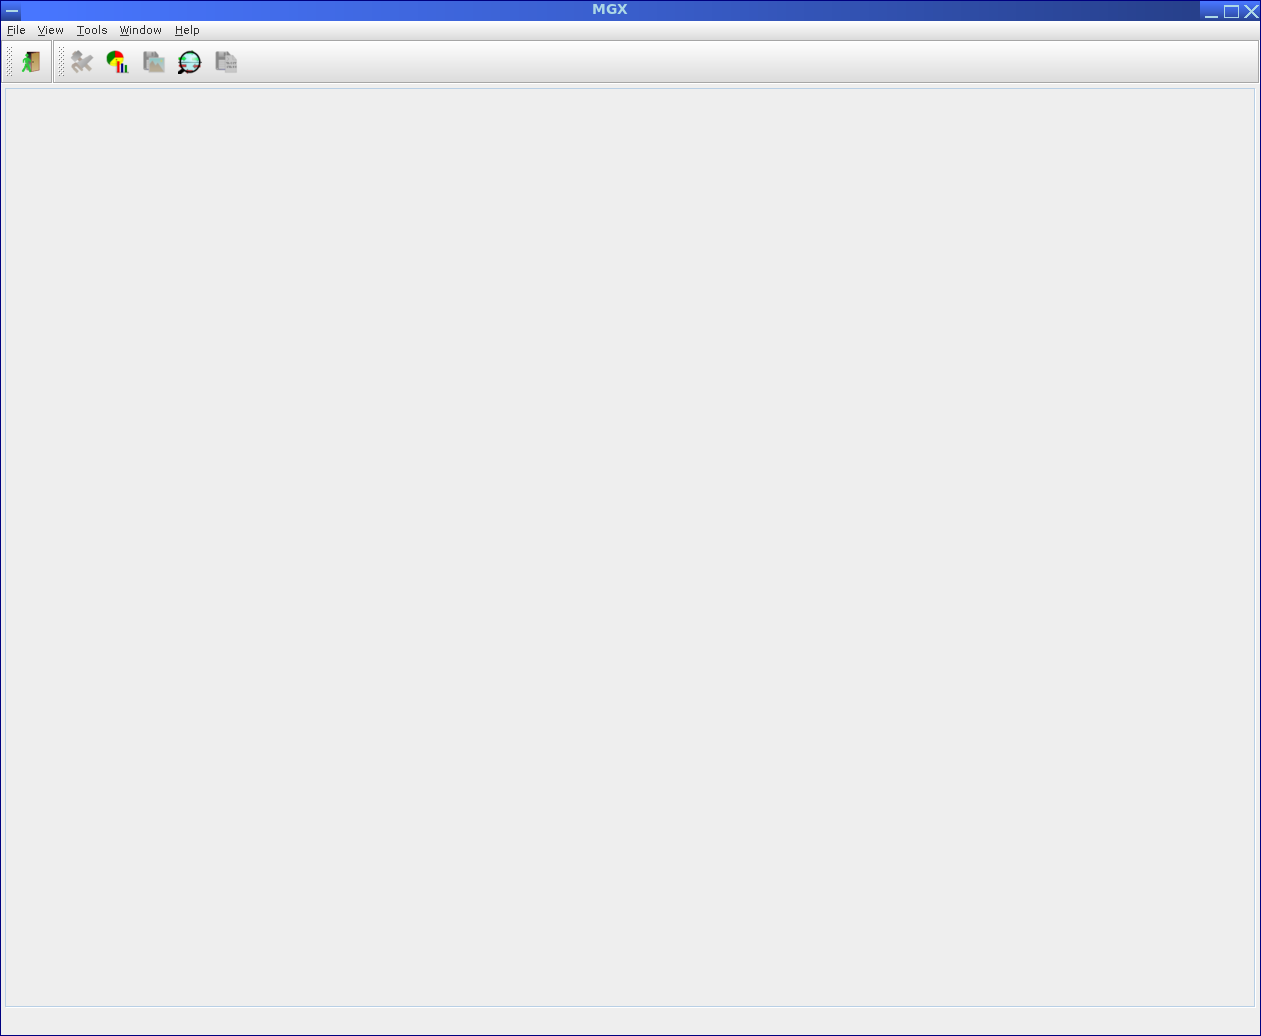
\includegraphics[width=\textwidth]{img/mgx/startup}
\caption[MGX client]{Screenshot of the client application right after startup.}
\label{startup}
\end{figure}

After installation, the MGX application is already preconfigured to connect to the 
MGX server instance hosted at CeBiTec, Bielefeld University. In case a different MGX server
should be used, the default server can be changed choosing Tools \textrightarrow Options from the menu
and navigating to the MGX server tab (\ref{config-site}). While the site name can be freely
chosen by the user, the server URL has to be entered as provided by the site administrators.

\begin{figure}[H]
\centering
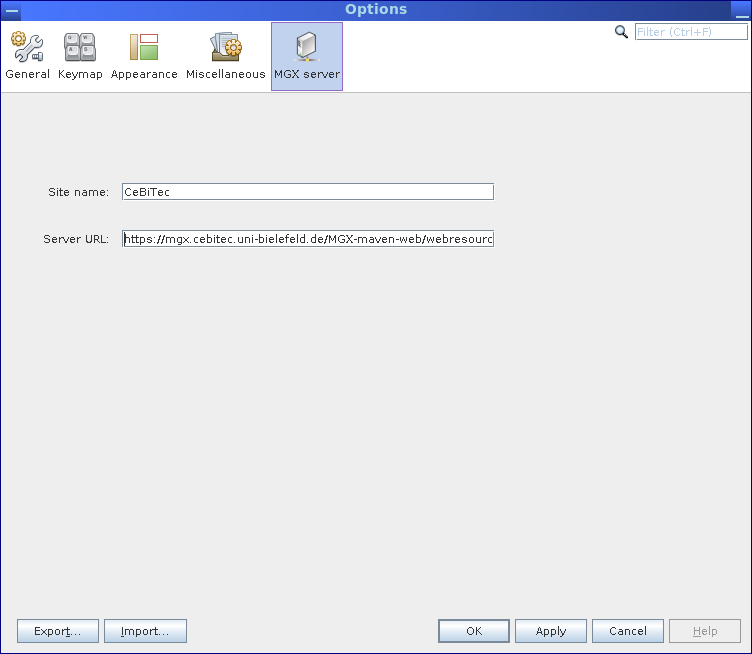
\includegraphics[width=.8\textwidth]{img/mgx/config-site}
\caption[Server configuration]{A different default server instance can optionally be configured in the MGX 
server tab, which is available from the Tools \textrightarrow Options menu.}
\label{config-site}
\end{figure}


\begin{figure}[H]
\centering
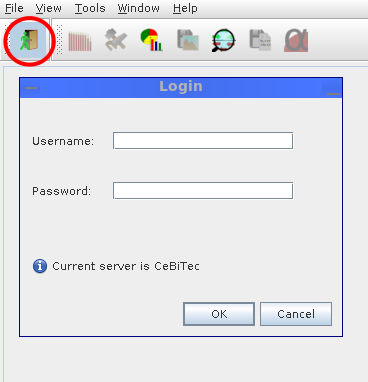
\includegraphics[width=.6\textwidth]{img/mgx/login}
\caption[Login screen]{The first button in the menu toolbar will bring up the login dialog, allowing to connect to the configured server; the login screen also reflects the name of the current server.}
\label{login-screen}
\end{figure}

All communication between the MGX user interface and the MGX server is encrypted using
the standardized SSL (Secure Sockets Layer) protocol, ensuring confidentiality of 
unpublished data and protecting the integrity of login credentials.
%\section{Browsing and exploring MGX projects}
After successfully logging in, a new window is automatically opened. The MGX Explorer window
lists all available projects a user is allowed to access, including both public as well as
private projects. Projects are easily opened or closed by simply expanding the corresponding
nodes in the Project Explorer window (\ref{projects}).\\

\begin{figure}[H]
\centering
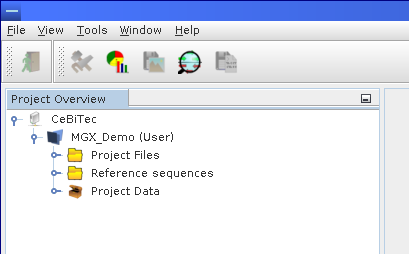
\includegraphics[width=.8\textwidth]{img/mgx/projects}
\caption[Project Explorer]{After successful login, the Project Explorer component will automatically open,
showing a list of MGX projects available to the current user. Shown is just one project, MGX\_Demo, with
``User'' access level indicated behind the project name.}
\label{projects}
\end{figure}

\begin{figure}[H]
\centering
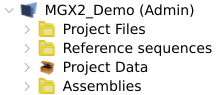
\includegraphics[width=.4\textwidth]{img/mgx/projstructure}
\caption[Project structure]{Divided into three different parts, a MGX projects offers
(from top to bottom) dedicated storage for files to be used by analysis pipelines, 
managed reference sequences (including annotation data, if available) and general
project data containing metadata as well as sequence datasets.}
\label{structure}
\end{figure}

Each project contains metagenome datasets as well as structured storage (\ref{structure}), where user-provided
databases can be uploaded to be used in custom analysis pipelines (Chapter \ref{custom}).

\section{Creating a new habitat}

New habitats are defined choosing ''Add habitat'' (\ref{addhabitat}) from the context menu of the ''Project Data''
node. This will bring up a wizard allowing to select the corresponding geographical location as well as
specifying a habitats name and biome type (\ref{habwiz}). In a second step, an optional description for this
habitat may be entered, as well.

\begin{figure}[H]
\centering
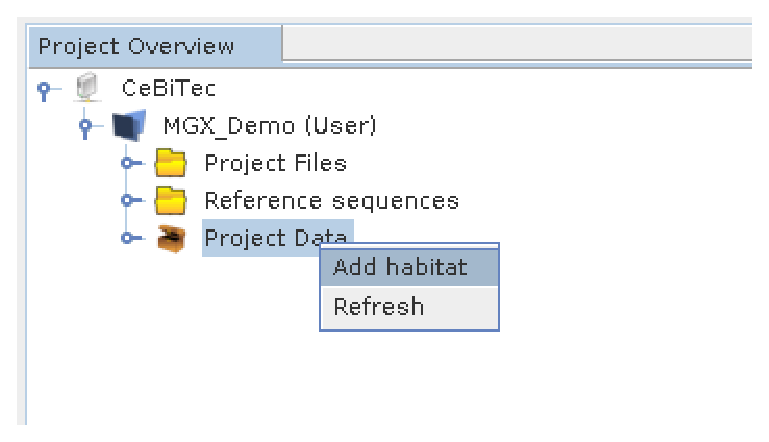
\includegraphics[width=.4\textwidth]{img/mgx/addhabitat}
\caption[Habitat creation]{A new habitat can be added selecting the appropriate entry from the context
menu of the ''Project Data'' node.}
\label{addhabitat}
\end{figure}

\begin{figure}[H]
\centering
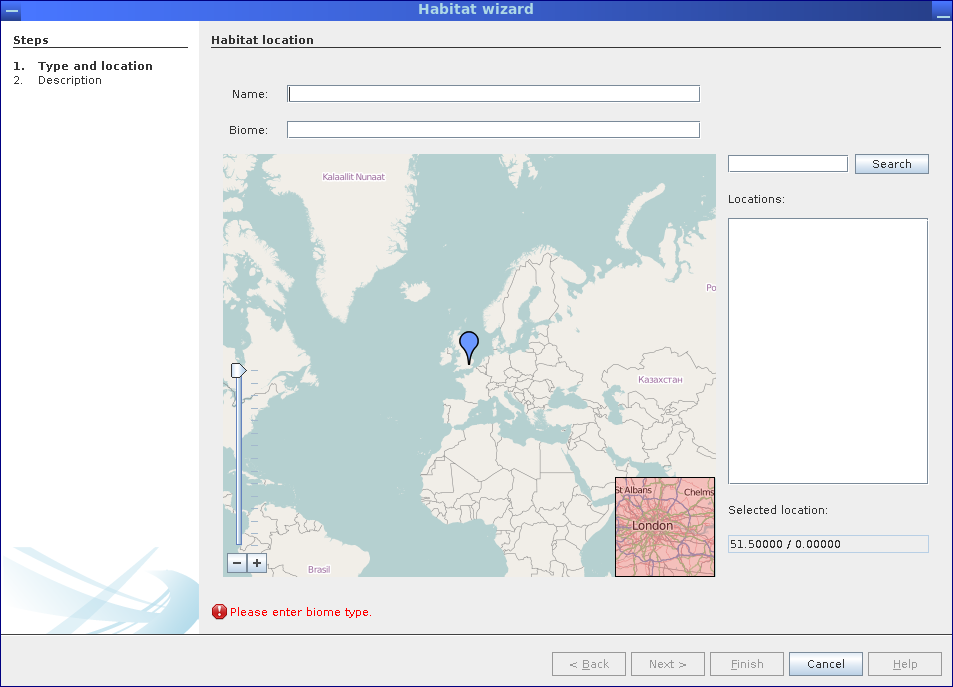
\includegraphics[width=.8\textwidth]{img/mgx/habwizard}
\caption[Habitat wizard]{The habitat wizard allows to define new habitats specifying their location, name and
biome type.}
\label{habwiz}
\end{figure}

\section{Creating new samples and DNA extracts}

Samples and DNA extracts are created in the same way as habitats, except that samples are defined for
habitats and DNA extracts are defined based on samples. Thus, the corresponding wizards are available
from the context menu of the ''Habitat'' and ''Sample'' nodes, respectively.

\begin{figure}[H]
\centering
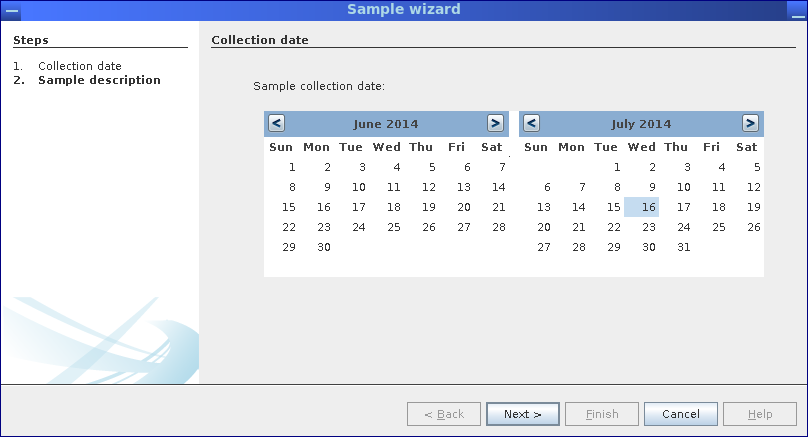
\includegraphics[width=.8\textwidth]{img/mgx/samplewiz1}
\caption[Sample wizard]{In the first step of the sample wizard, the sampling date is selected.}
\label{samplewiz1}
\end{figure}

\begin{figure}[H]
\centering
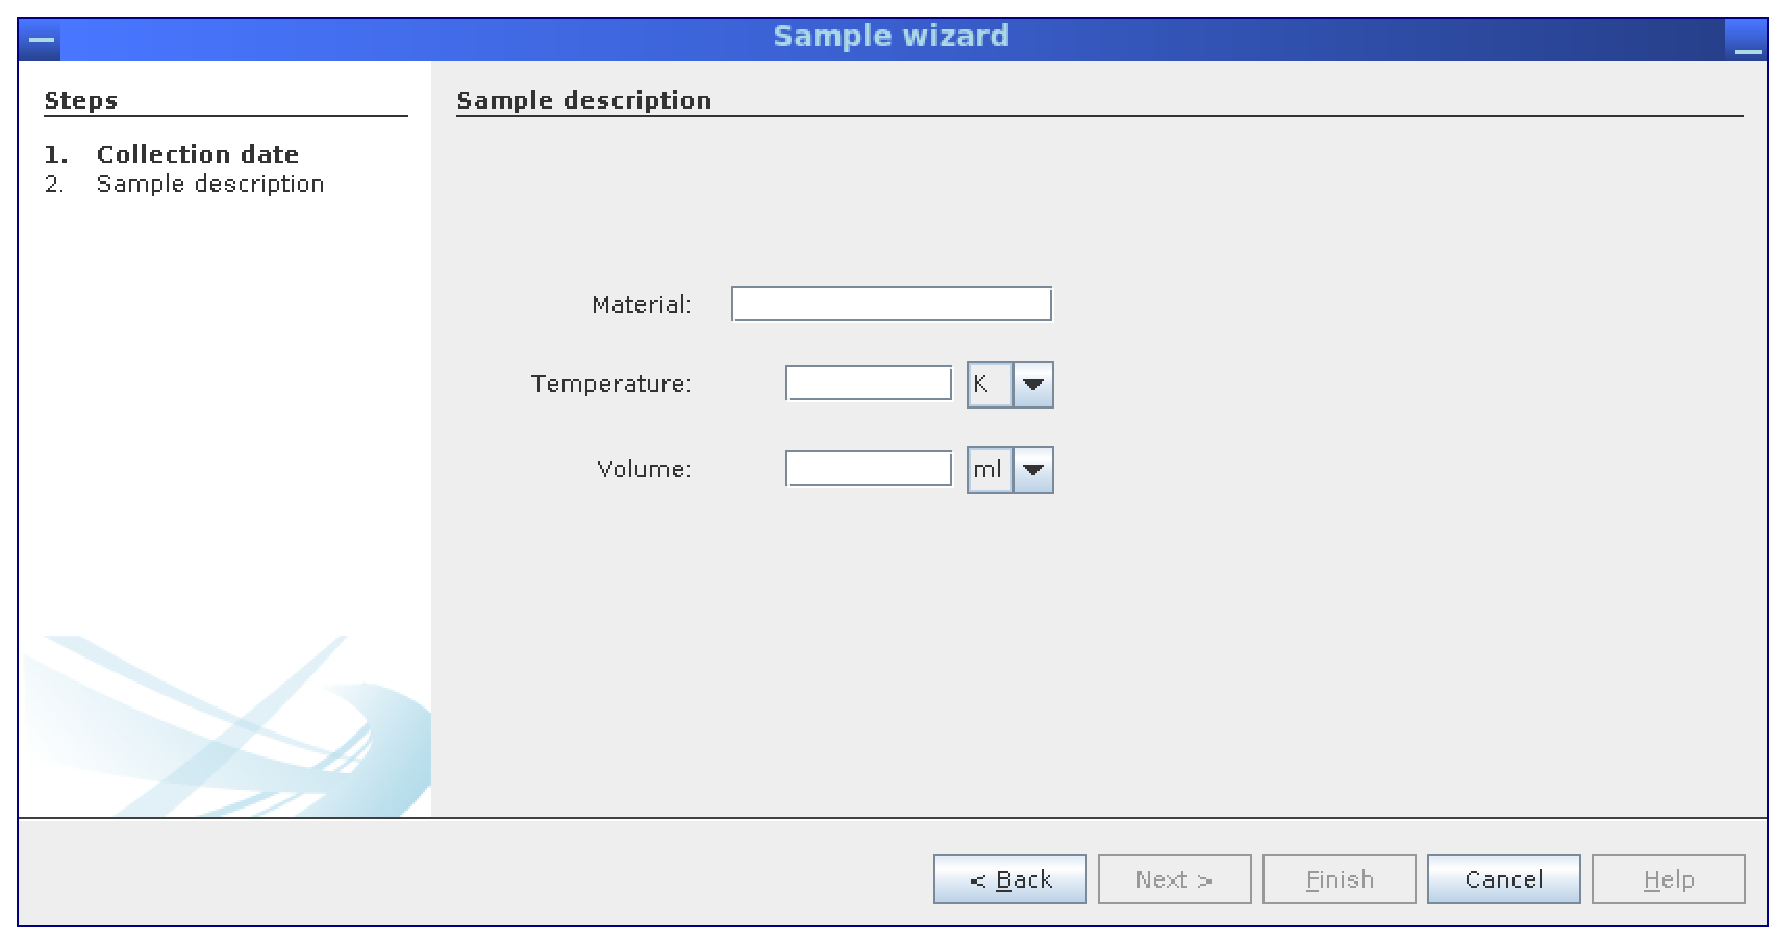
\includegraphics[width=.8\textwidth]{img/mgx/samplewiz2}
\caption[Sample wizard]{In the second step, the sampled material as well as temperature and sampled volume/weight
need to be entered.}
\label{samplewiz2}
\end{figure}

\begin{figure}[H]
\centering
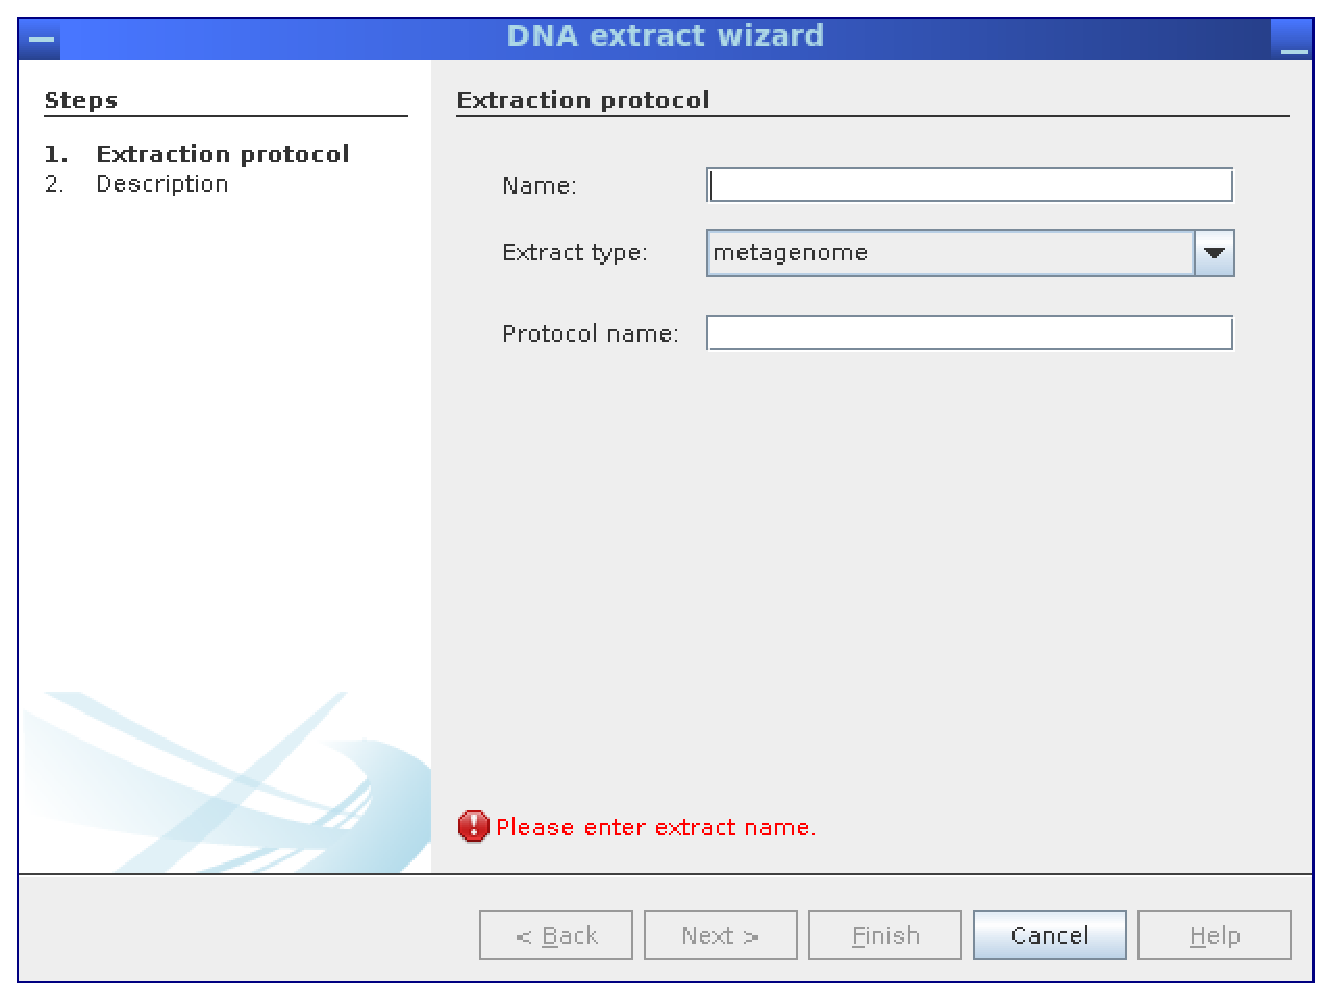
\includegraphics[width=.8\textwidth]{img/mgx/extractwiz1}
\caption[DNA extract wizard]{The DNA extract wizard allows to specify the type of DNA extract (metagenome, 
metatranscriptome, amplicon) and protocols used to extract the DNA.}
\label{extractwiz1}
\end{figure}

\begin{figure}[H]
\centering
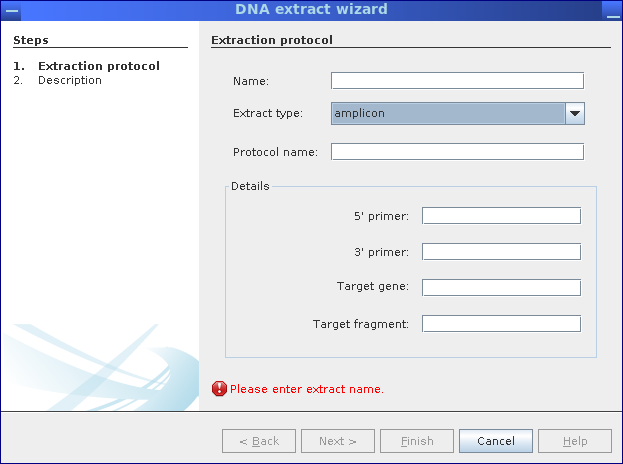
\includegraphics[width=.8\textwidth]{img/mgx/extractwiz2}
\caption[DNA extract wizard]{Depending on DNA extract type, additional data can be provided; for amplicons, primer
names and the corresponding target gene (fragment) can be entered, for metatranscriptomes, the type of RNA depletion
methods can be selected.}
\label{extractwiz2}
\end{figure}

\section{Importing sequence data}

\begin{figure}[H]
\centering
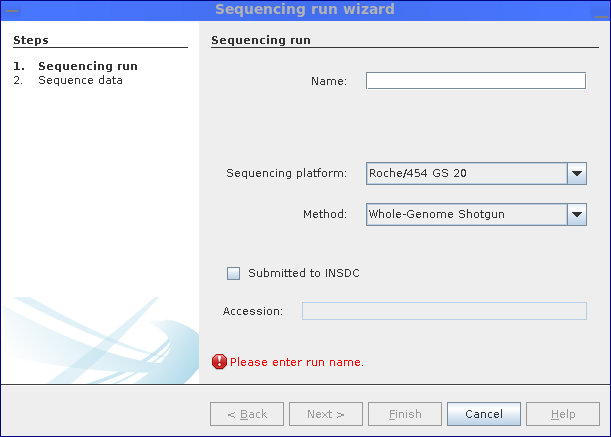
\includegraphics[width=.8\textwidth]{img/mgx/runwiz1}
\caption[Sequence import]{Before sequence data can be uploaded, the employed sequencing platform and technology have 
to be specified; for data already submitted to or obtained from public INSDC repositories (e.g. NCBI, EBI, DDBJ), the
corresponding accession number can be stored, as well.}
\label{dnawiz1}
\end{figure}

\begin{figure}[H]
\centering
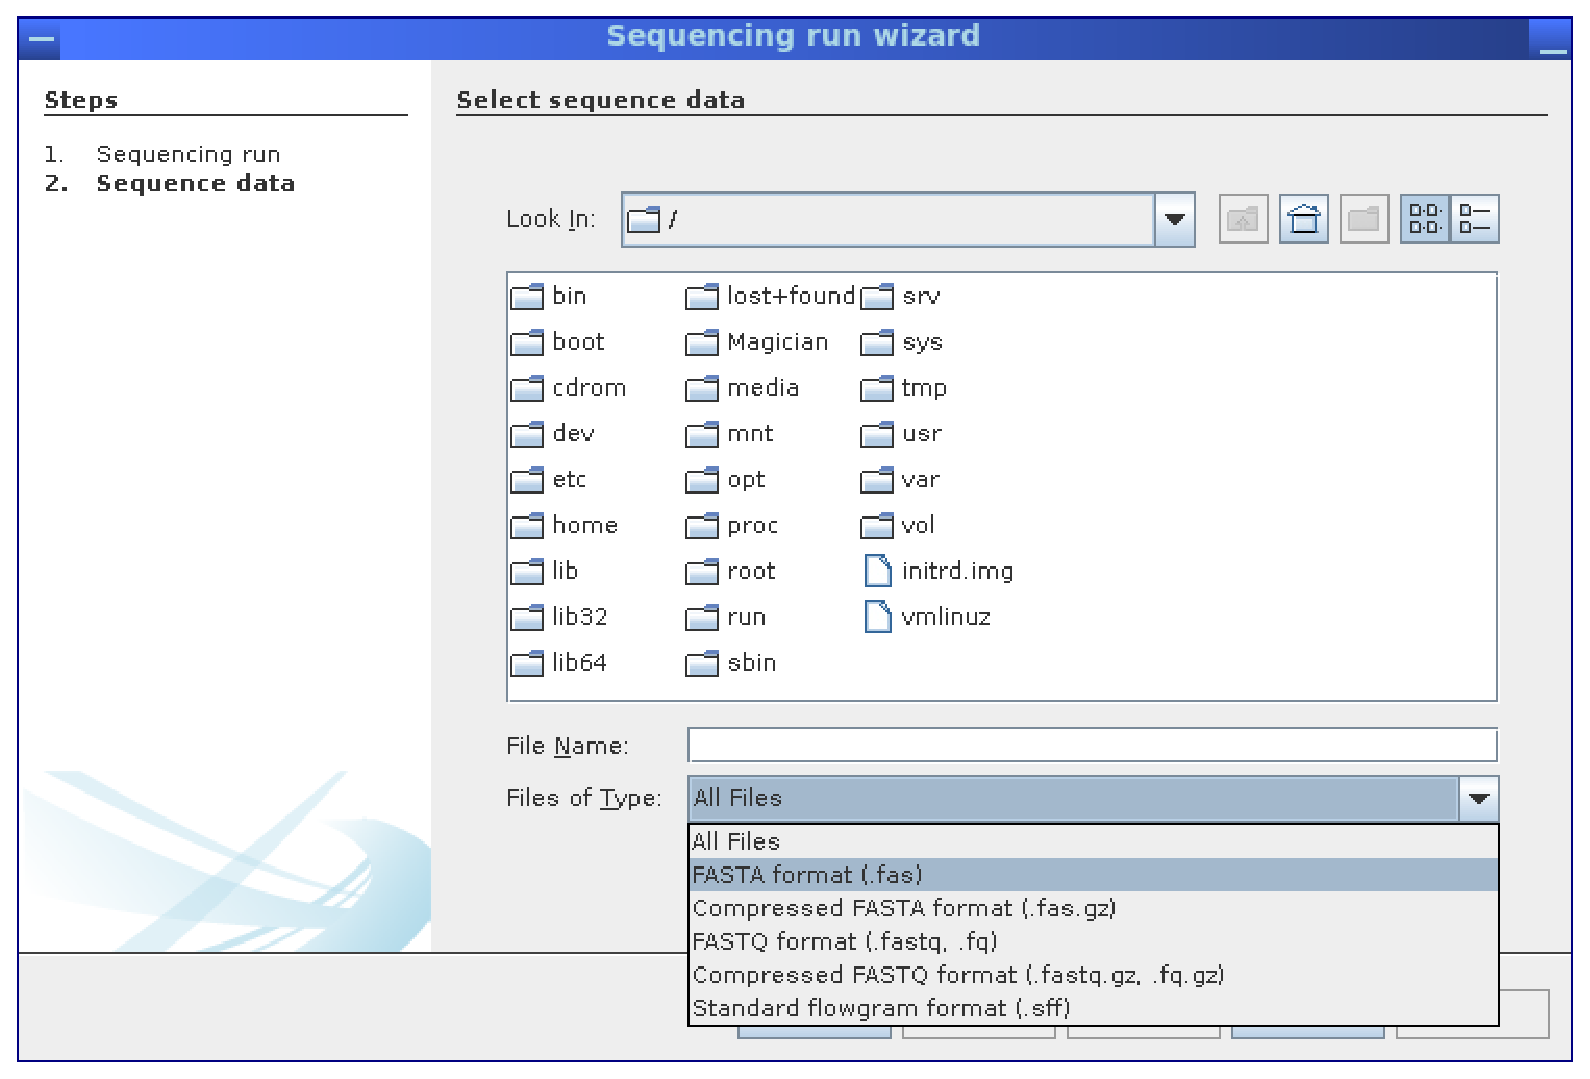
\includegraphics[width=.8\textwidth]{img/mgx/runwiz2}
\caption[Sequence import]{Finally, the file containing the sequence data is selected; MGX supports all commonly used
file formats such as FASTA, FASTQ, or SFF.}
\label{dnawiz2}
\end{figure}

\section{Quality control}

\begin{figure}[H]
\centering
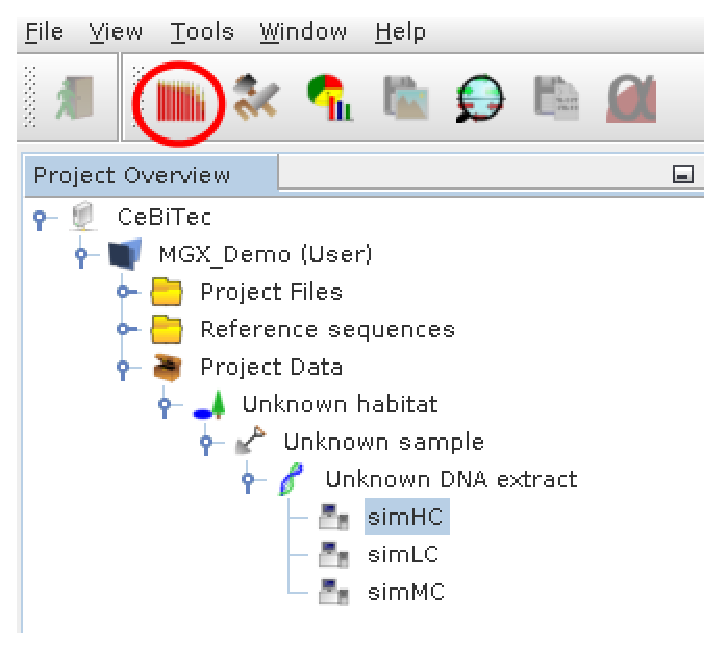
\includegraphics[width=.6\textwidth]{img/mgx/QCopen}
\caption[Quality control]{After selecting a sequencing run object, the Quality Control component can be opened
from its menubar icon (red circle).}
\label{qcopen}
\end{figure}

After sequence import, Quality control reports generated within MGX should be inspected (\ref{qcopen}) before proceding with data analysis.
MGX currently offers three types of QC reports: Distribution of GC content, sequence length
and nucleotide distribution within the DNA sequences. Those can be used to evaluate overall
sequence data quality and check for possible signs of contamination.
For demonstration purposes, data shown relates to the artificial \textbf{simHC} metagenome dataset created by the
FAMeS\cite{SIMMETA} project. The actual sequence data is publicly available and can be obtained from
the FAMeS web site (\url{http://fames.jgi-psf.org/Retrieve_data.html}).

\begin{figure}[H]
\centering
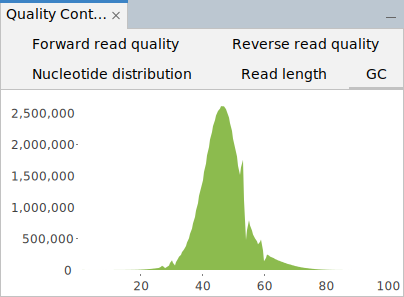
\includegraphics[width=.6\textwidth]{img/mgx/QCgc}
\caption[Quality control]{GC distribution of the simHC dataset.}
\label{qc1}
\end{figure}

\begin{figure}[H]
\centering
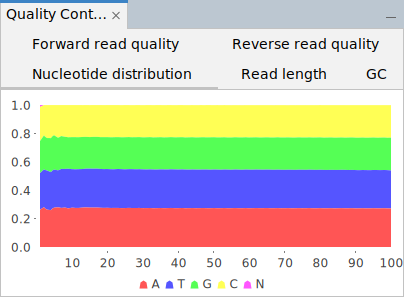
\includegraphics[width=.6\textwidth]{img/mgx/QCnuc}
\caption[Quality control]{Nucleotide distribution of the simHC dataset. A high fraction of uncalled bases
is apparent from the chart.}
\label{qc2}
\end{figure}

\begin{figure}[H]
\centering
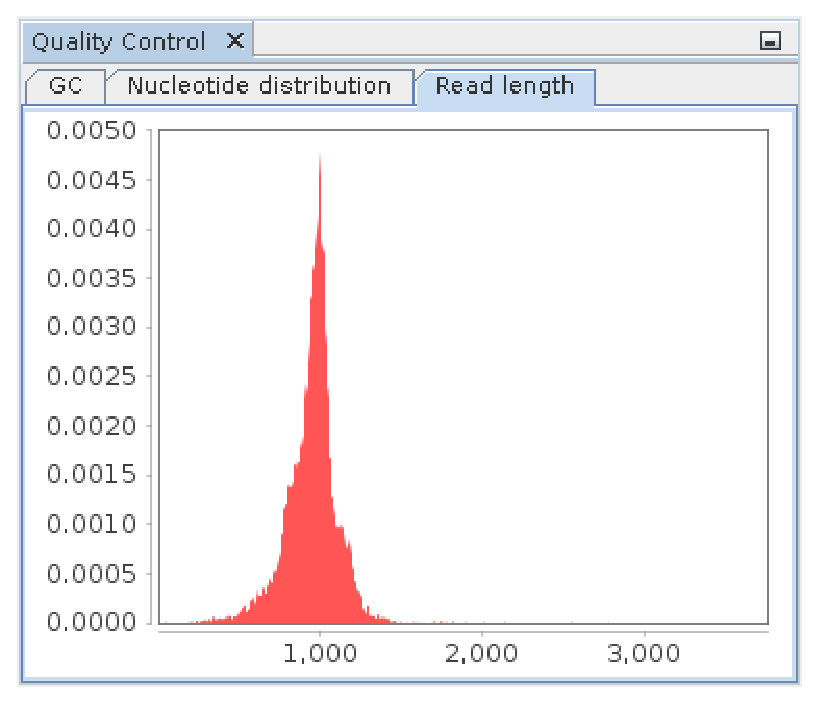
\includegraphics[width=.6\textwidth]{img/mgx/QCreadlen}
\caption[Quality control]{Read length distribution of the simHC dataset. }
\label{qc3}
\end{figure}

\begin{figure}[H]
        \centering
        \begin{subfigure}[b]{0.3\textwidth}
                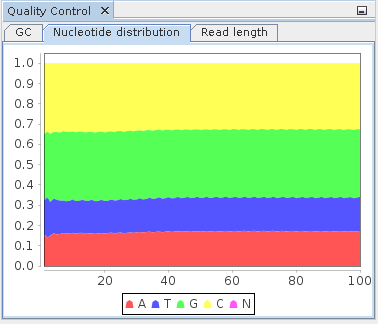
\includegraphics[width=\textwidth]{img/mgx/highGCnucl}
                \caption{High-GC (65\%) data}
        \end{subfigure}%
        \begin{subfigure}[b]{0.3\textwidth}
                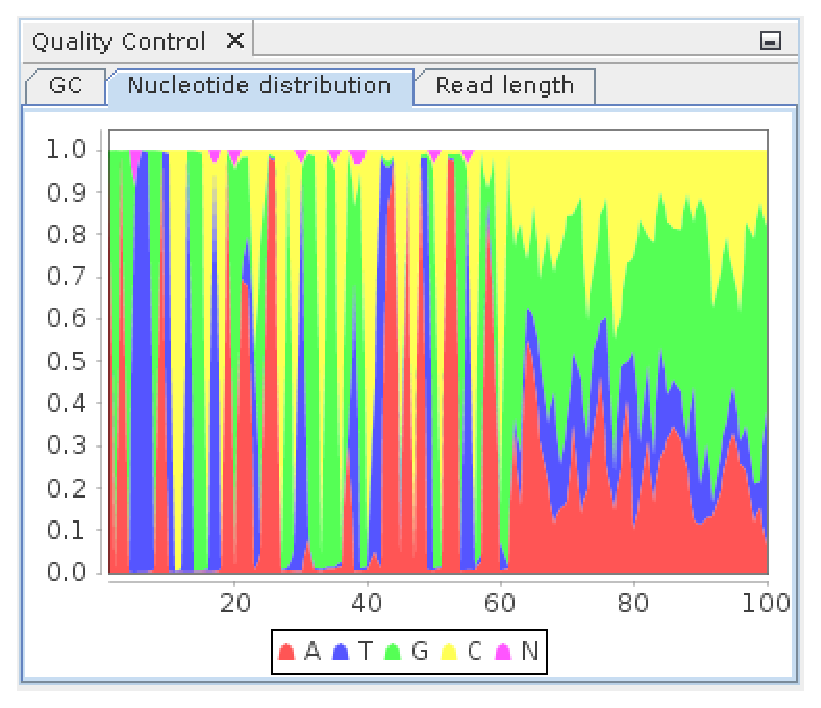
\includegraphics[width=\textwidth]{img/mgx/ampliconNucl}
                \caption{Amplicon data}
        \end{subfigure}
        \begin{subfigure}[b]{0.3\textwidth}
                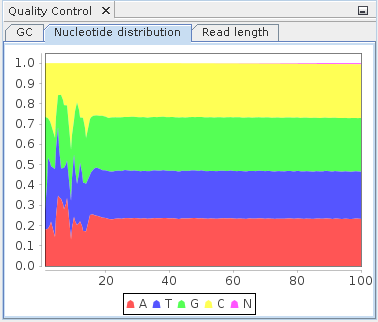
\includegraphics[width=\textwidth]{img/mgx/adapterNucl}
                \caption{Adapter residue}
        \end{subfigure}
        \caption{Nucleotide distribution examples.}
  \label{qc4}
\end{figure}

Depending on the kind of sequence data, different patterns might emerge (\ref{qc4}),
which might or might not warrant any further action. While small amounts of e.g. 
adapter residue are sometimes encountered and might be considered acceptable, it is up to the
individual researcher to check back with their sequencing provider and ask for
adapter sequences to execute additional trimming.

\section{Defining and executing analysis jobs}

\begin{figure}[H]
\centering
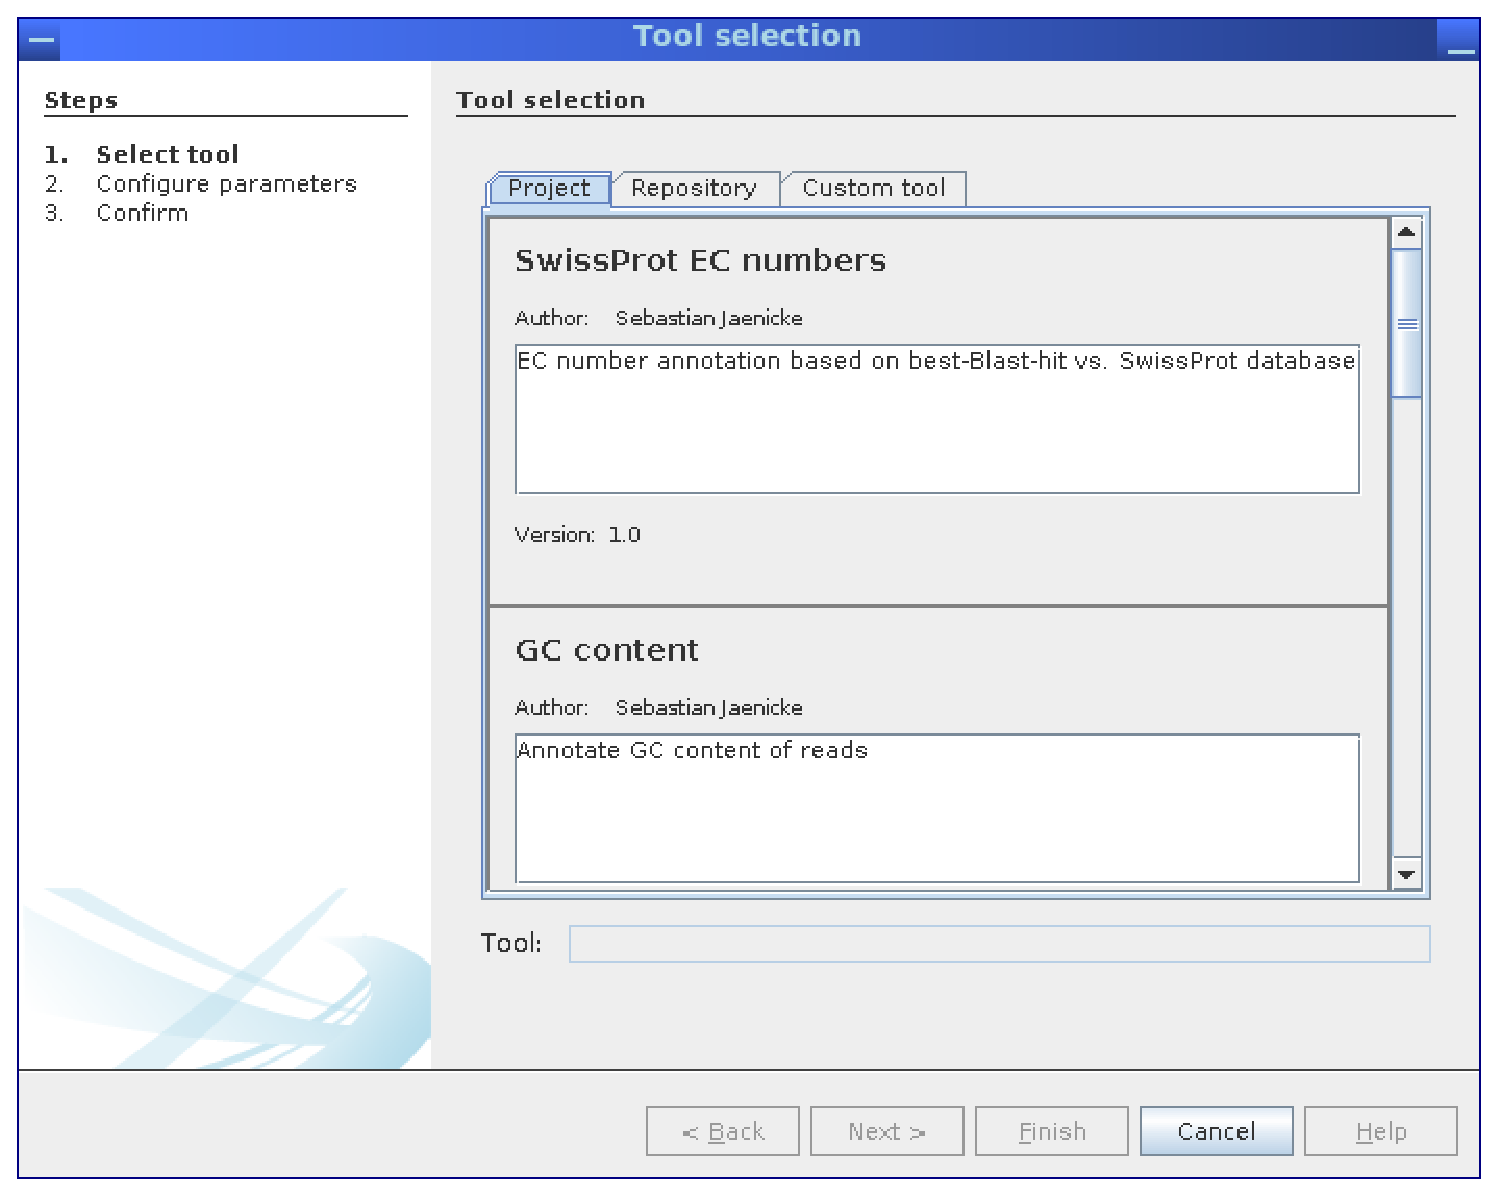
\includegraphics[width=.8\textwidth]{img/mgx/analysiswiz1}
\caption[Analysis selection]{Analysis pipelines can be selected from the corresponding
MGX project itself, from the repository of public pipelines provided by the server, or,
a custom workflow can be uploaded and executed.}
\label{anawiz1}
\end{figure}

All analysis pipelines can be started from the context menu of the metagenome dataset to be analyzed, provided
the user has been granted at least ``User'' level access. First,
the user can choose the desired pipeline from the project itself, from the pipeline repository hosted on the
MGX server, or upload an own pipeline implementation (\ref{anawiz1}). Subsequently, analysis parameters
can be reviewed and adapted (\ref{anawiz2}) before submitting an analysis.

\begin{figure}[H]
\centering
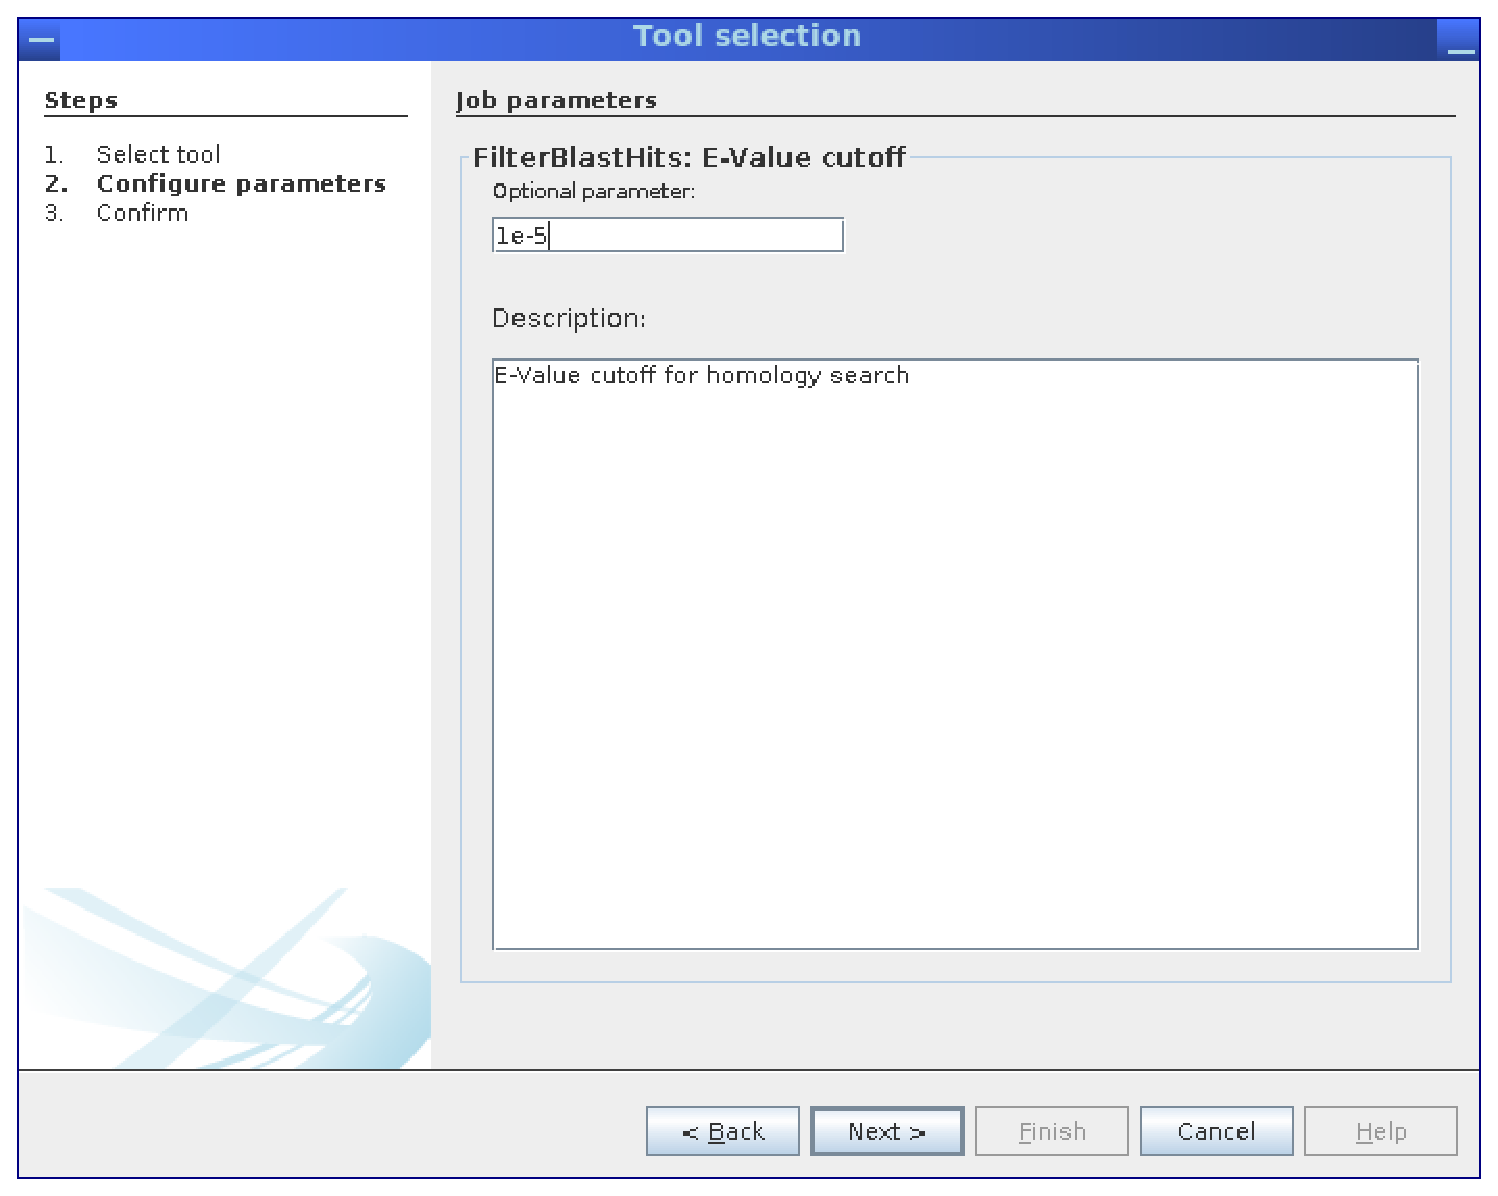
\includegraphics[width=.8\textwidth]{img/mgx/analysiswiz2}
\caption[Analysis parameters]{The wizard allows to inspect and adapt parameters for the selected pipeline. The actual
number of steps depends on the number of parameters available for customization.}
\label{anawiz2}
\end{figure}

\begin{figure}[H]
\centering
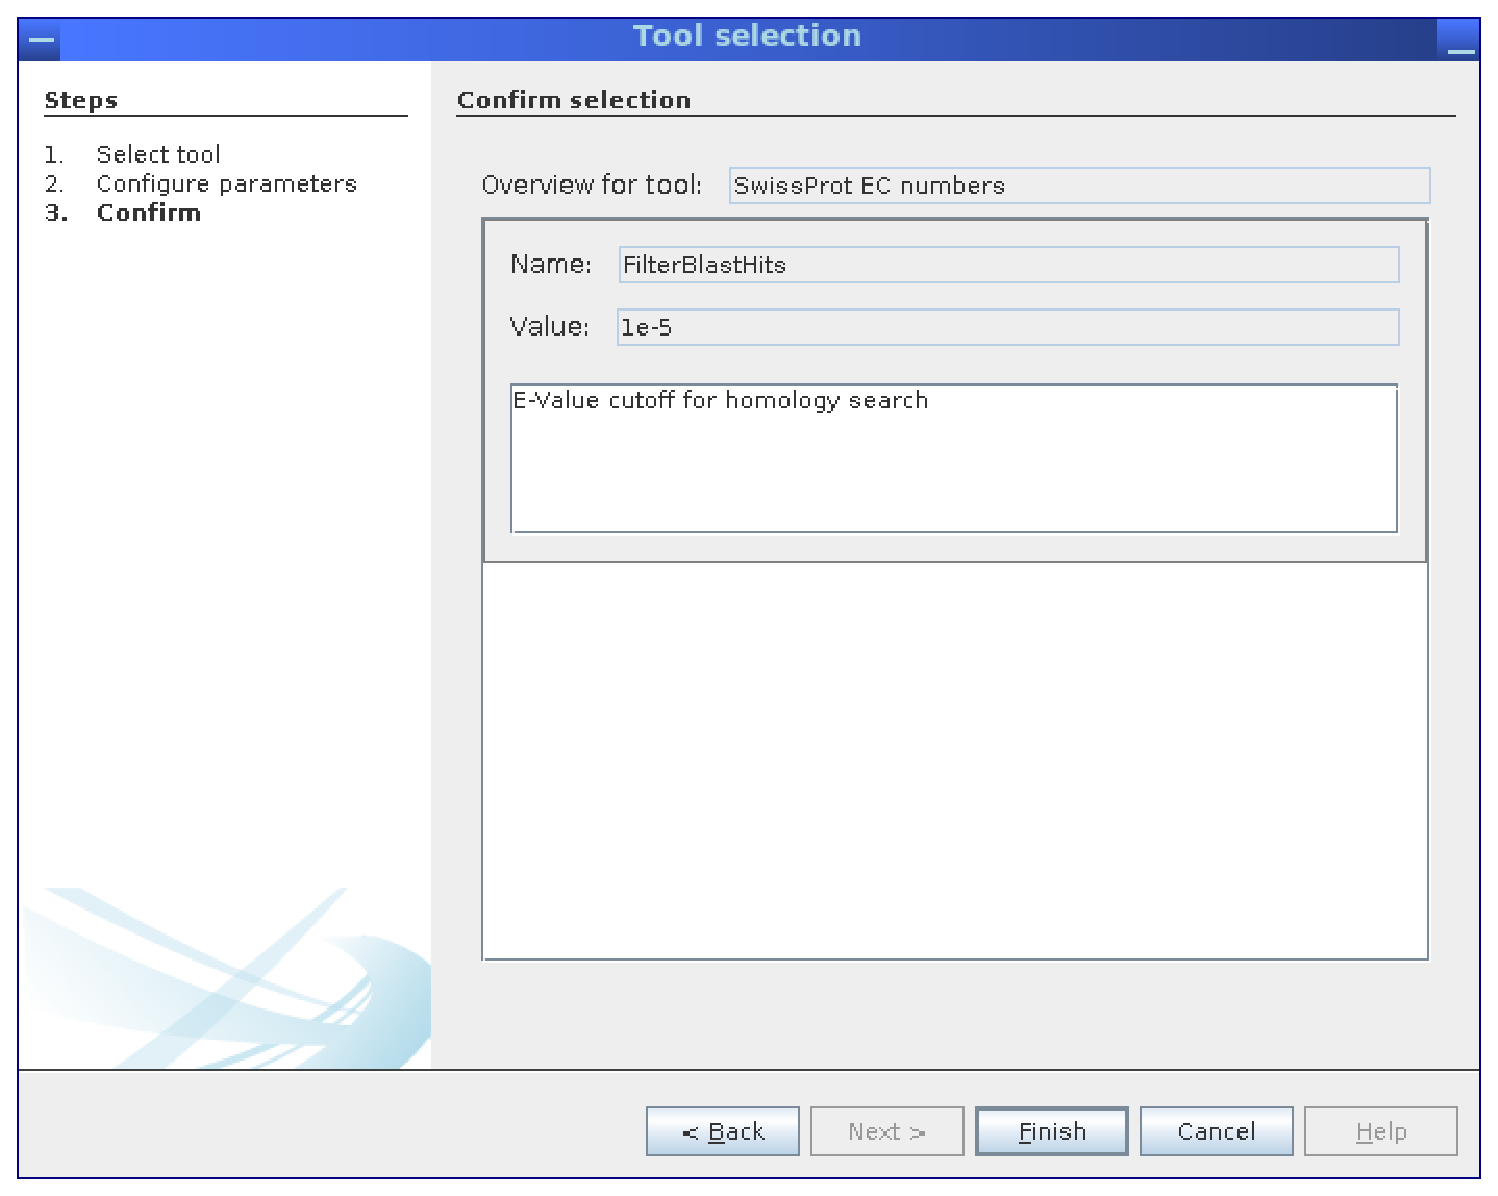
\includegraphics[width=.8\textwidth]{img/mgx/analysiswiz3}
\caption[Parameter overview]{Before executing an analysis pipeline, a final overview of all parameters is shown. Once
confirmed, the pipeline is submitted and scheduled for execution on the MGX server. Here, the selected pipeline has
only one single parameter.}
\label{anawiz3}
\end{figure}

\subsection{Monitoring job progress}

\begin{figure}[H]
\centering
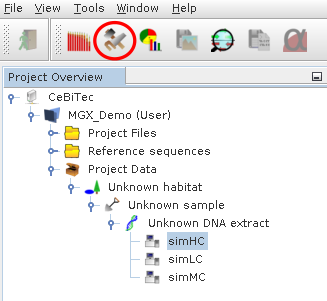
\includegraphics[width=.6\textwidth]{img/mgx/JobMonOpen}
\caption[Job monitor]{The Job Monitor component can be opened using its icon in the toolbar.}
\label{jobmon1}
\end{figure}

\begin{figure}[H]
\centering
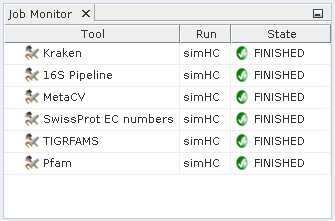
\includegraphics[width=.6\textwidth]{img/mgx/JobMon}
\caption[Job monitor]{The Job Monitor provides an overview of job states. Depending on context, all jobs
within a MGX project or only jobs for a single dataset will be displayed.}
\label{jobmon2}
\end{figure}

The Job Monitor component is provided to inspect the state of jobs present within a MGX project.
It can be opened from the toolbar (\ref{jobmon1} )and will display the state of jobs scheduled for execution,
currently running or already finished (\ref{jobmon2}). In addition, it can also be used to delete jobs and
corresponding analysis results when no longer needed. Depending on the selected item in the
Project Explorer, the Job Monitor will by default display all jobs within a project; if a single
sequencing run is selected, only jobs for this dataset will be shown.

\section{Visualization of results}

\begin{figure}[H]
\centering
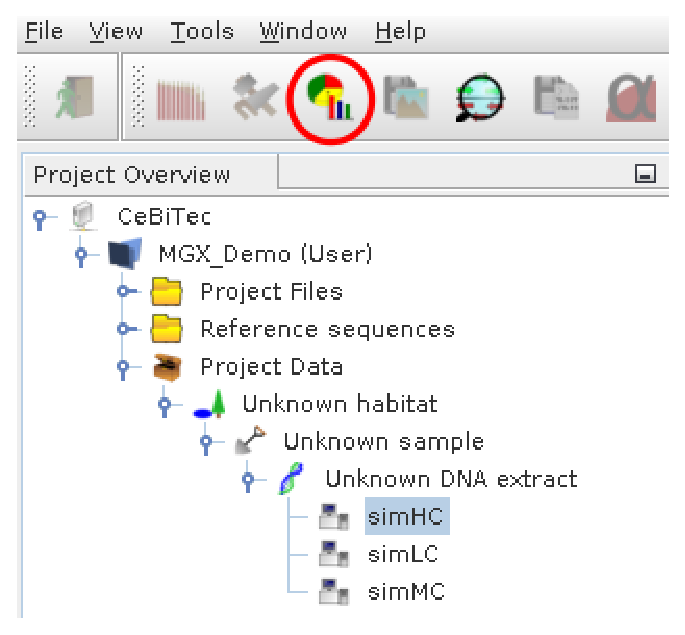
\includegraphics[width=.6\textwidth]{img/mgx/VizOpen}
\caption[Visualization]{Icon for the visualization module.}
\label{viz1}
\end{figure}

\begin{figure}[H]
\centering
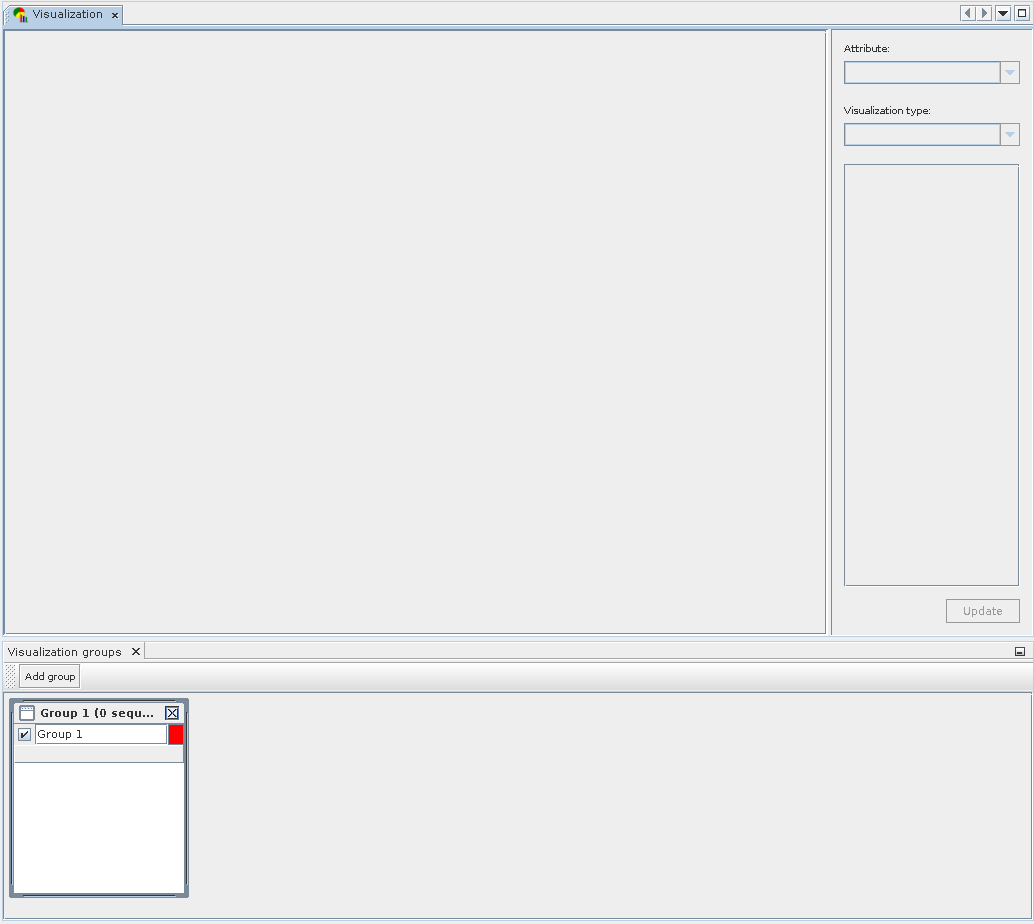
\includegraphics[width=.8\textwidth]{img/mgx/VizComponent}
\caption[Visualization components]{Components of the visualization module. The bottom window is
used to create and define groups, while the top window allows to select result and visualization
type, customize options and display the final chart.}
\label{viz2}
\end{figure}

The visualization component actually consists of two separate windows (\ref{viz2}). The Group
Window is located at the bottom and used to create, name and define groups used for data display.
Sequencing runs can be added to individual groups using \textit{Drag and Drop}. While any
sequencing run can be present in several groups at the same time, it is not possible to add
it to a group more than once. Groups may be assigned a name, their display color can be chosen
by the user, and they may be temporarily excluded from display.\\
The main visualization window is shown at the top; once sequencing runs are added or changed, 
the type of analysis result to be shown can be chosen on the top right. Afterwards, the desired
visualization type is selected and may be customized, as well.

\begin{figure}[H]
\centering
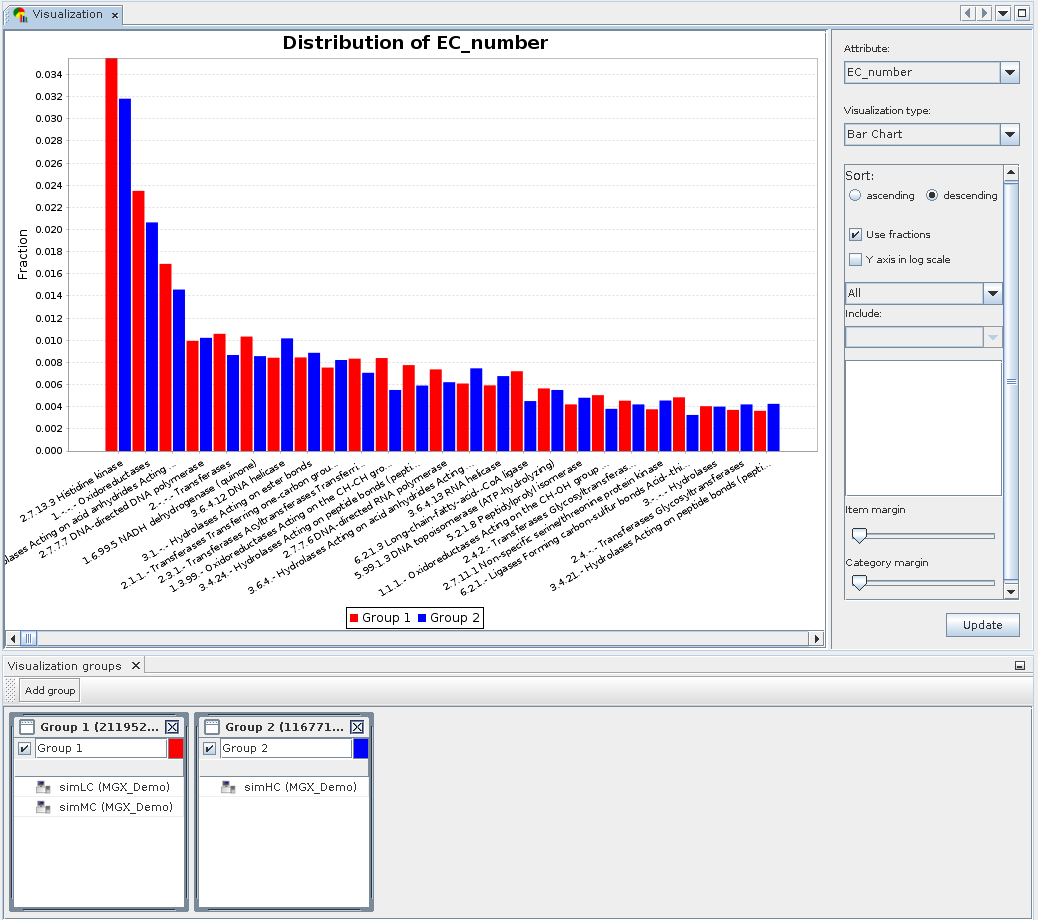
\includegraphics[width=\textwidth]{img/mgx/VizDemo}
\caption[Visualization example]{Visualization example displaying a bar chart for two groups.}
\label{viz3}
\end{figure}

Figure \ref{viz3} shows a simple visualization example. Two groups were defined containing the simLC and simMC metagenomes
in the first and the simHC metagenome in the second group. The main visualization window shows a bar chart
generated for these groups based on assigned EC numbers. To account for differences in dataset size, both
groups are normalized to fractions.

\begin{figure}[H]
\centering
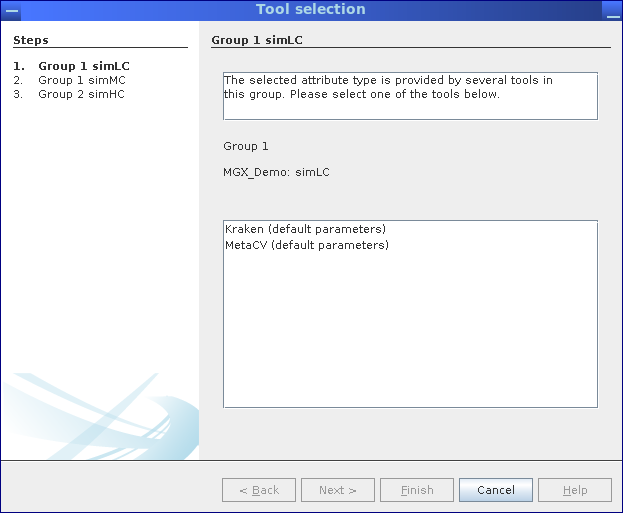
\includegraphics[width=.8\textwidth]{img/mgx/ConflictResolver}
\caption[Job selection]{In case a result is provided by more than one job, e.g. different taxonomic assignment methods,
a dialog allows to select between jobs. In this example, taxonomic assignments are provided by MGX pipelines employing Kraken\cite{KRAKEN}
as well as MetaCV\cite{METACV}.}
\label{viz4}
\end{figure}

Whenever a selected result type is provided by more than one analysis job, an interactive dialog allow the user to
review possible jobs and select one (\ref{viz4}). This scenario will occur when a tool is executed several 
times with different parameters, or when different taxonomic classifiers were used to analyse a dataset.

\subsection{Exporting sequences}

\begin{figure}[H]
\centering
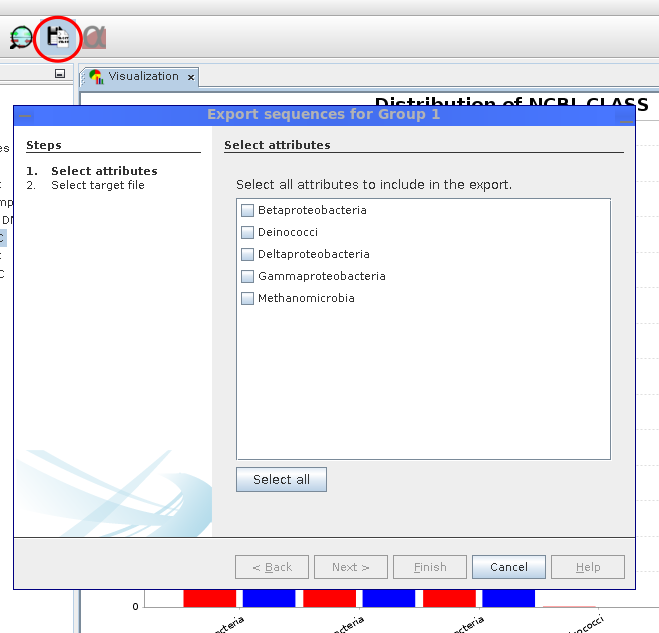
\includegraphics[width=.8\textwidth]{img/mgx/SeqExport}
\caption[Exporting sequences]{Sequences can be exported for each group individually. The user can freely choose
which attributes should be included.}
\label{seqexp}
\end{figure}

The sequence export wizard allows to export sequences conditionally based on analysis results. For each
visualization group, it is possible to choose the attributes for which sequences should be obtained (\ref{seqexp}).
Sequences are subsequently downloaded from the MGX server and saved in FASTA format files for each group.


\subsection{Biodiversity indices}

\begin{figure}[H]
\centering
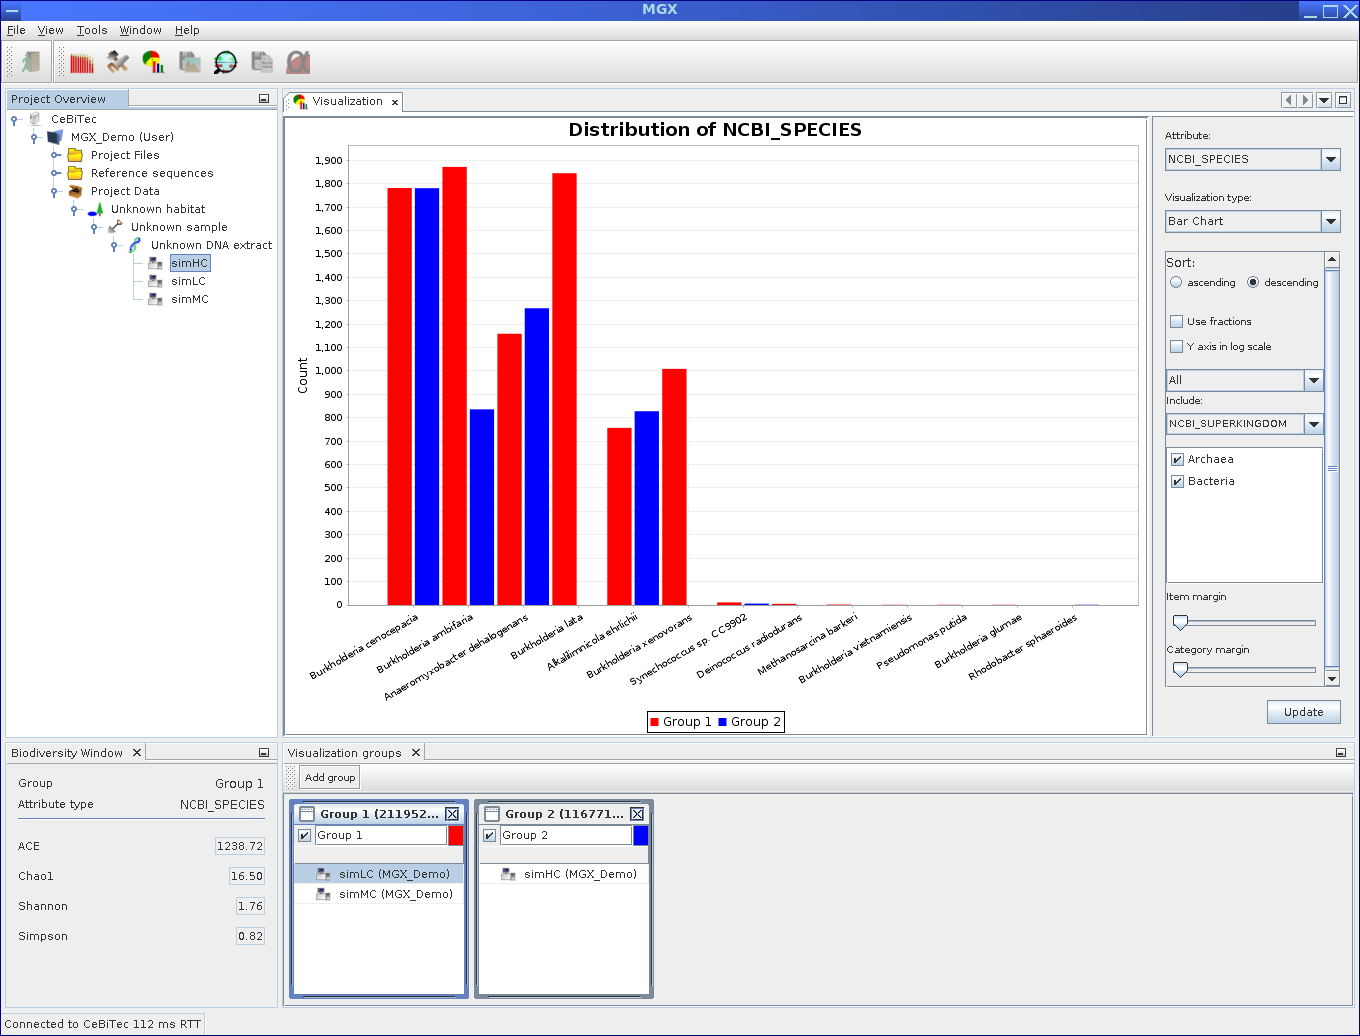
\includegraphics[width=\textwidth]{img/mgx/BioDiversity}
\caption[Biodiversity]{Biodiversity indices (bottom left) such as ACE or Shannon are computed for the currently
selected visualization group.}
\label{biodiv}
\end{figure}

The visualization module features another component used to display commonly used biodiversity indices, such as
the ACE, Shannon\cite{SHANNON}, Chao1\cite{DIVERSITY} and Simpson\cite{SIMPSON} indices. The component will automatically show the index values for the
currently selected visualization group based on the chosen attribute type (\ref{biodiv}).

\section{Reference mapping}

\begin{figure}[H]
\centering
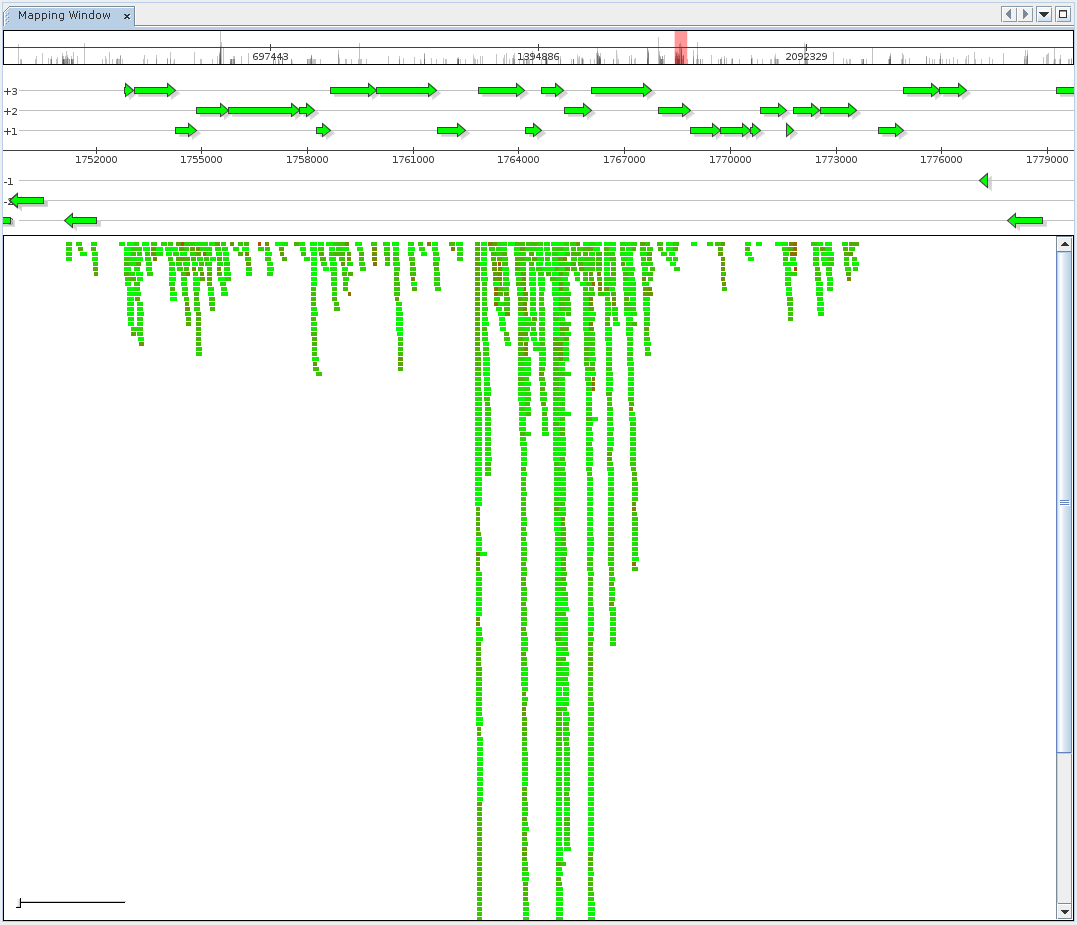
\includegraphics[width=\textwidth]{img/mgx/RefMapping}
\caption[Reference mapping]{The reference mapping component showing alignment results for a metatranscriptome dataset mapped to the reference genome of one of the dominant organisms. From top to bottom, the component displays a) navigation and coverage histogram, b) currently selected interval and c) aligned DNA sequences for the interval. Color coding refers to relative sequence identity.}
\label{refmap}
\end{figure}

Alignment of metagenome or metatranscriptome data to reference sequences of known origin allows researchers to evaluate
relative identity between metagenome sequences and the actual strain or to obtain an overview of gene expression within
a meta-transcriptome. MGX currently provides predefined pipelines employing FR-HIT\cite{FRHIT} and Bowtie 2\cite{BOWTIE}. The reference mapping 
component is provided to inspect and browse alignment results.

\section{Search}

\begin{figure}[H]
\centering
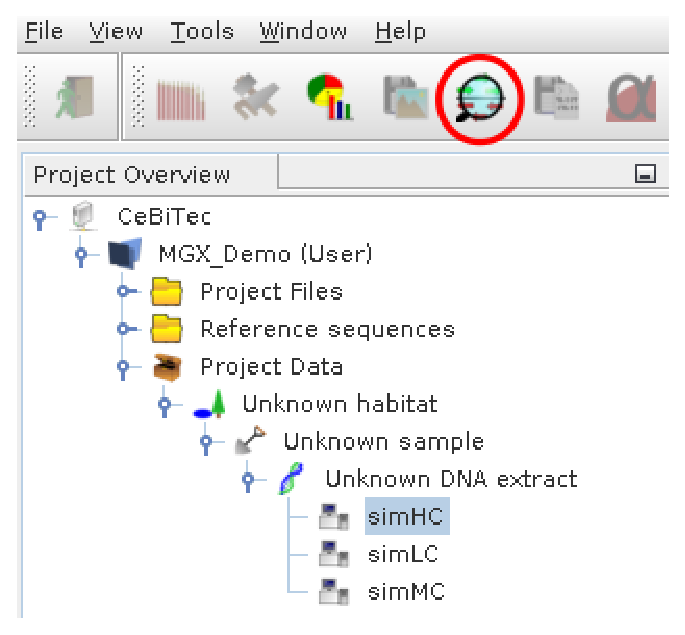
\includegraphics[width=.5\textwidth]{img/mgx/SearchOpen}
\caption[Metagenome search]{Icon for the metagenome search component.}
\label{search1}
\end{figure}

\begin{figure}[H]
\centering
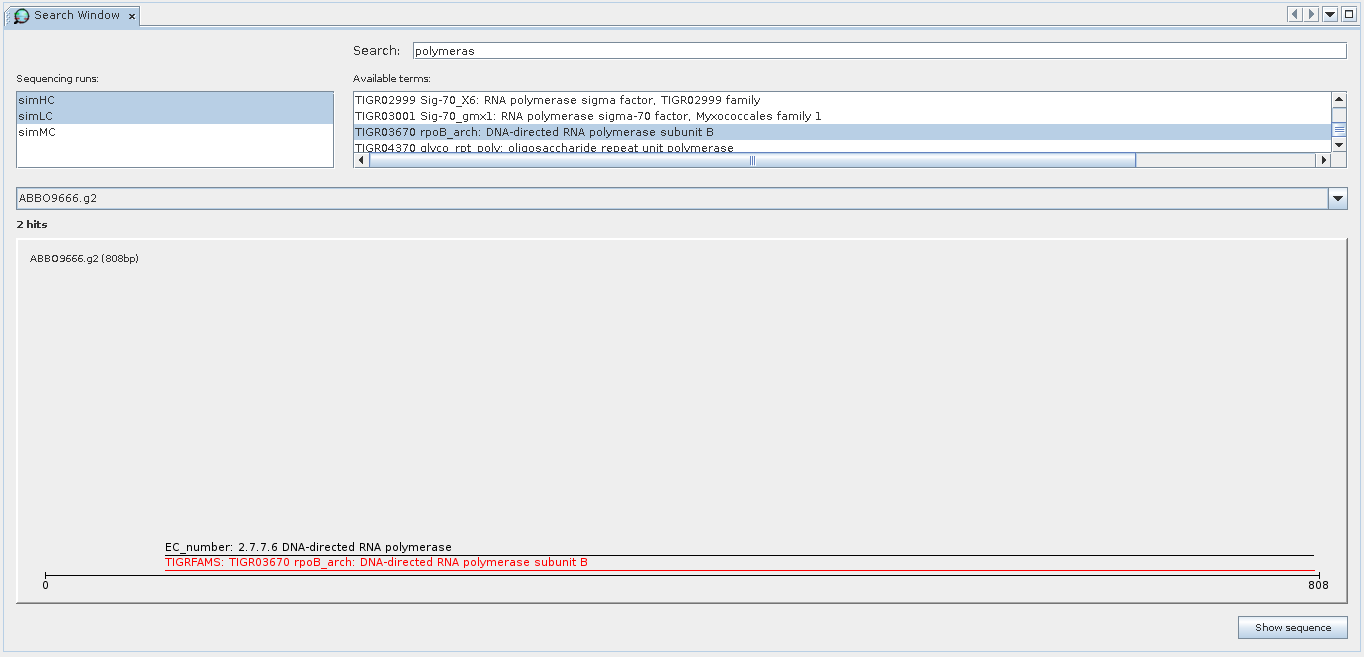
\includegraphics[width=.9\textwidth]{img/mgx/SearchTC}
\caption[Metagenome search]{Search component showing results for the term ``polymeras''. The search was performed
within the select metagenomes simHC and simLC (top left); the bottom part shows an individual sequence identified
by the search. Search results are displayed together with all other attributes available for a sequences, thus allowing
to identify co-occurence of results.}
\label{search2}
\end{figure}


TODO



\chapter{Implementing custom analysis pipelines}
\label{custom}

All offered analysis tools provided by the MGX platform are implemented as workflows
for the Conveyor\cite{CONVEYOR} workflow engine developed by B. Linke. Within Conveyor,
tools are provided as so-called ''nodes'', which resemble individual processing steps
and which are used to implement novel analysis methods by simply arranging and connecting
them into a larger workflow. Conveyor currently includes plugins providing typical
bioinformatics tools like BLAST or HMMer, but has recently been extended with dedicated
plugins aimed at metagenome analysis, like MetaCV, MetaPhyler or MetaPhlAn, which all
perform taxonomic analysis.
A dedicated Conveyor plugin provides access to MGX data structures, thereby enabling the
analysis of metagenomes stored in the MGX system with processing tools provided by Conveyor
itself.
While workflow definitions are stored in a XML-based format, a graphical user interface,
the Conveyor Designer (\ref{designer}), enables users to implement new analysis by simply
placing and connecting nodes.

\begin{figure}[H]
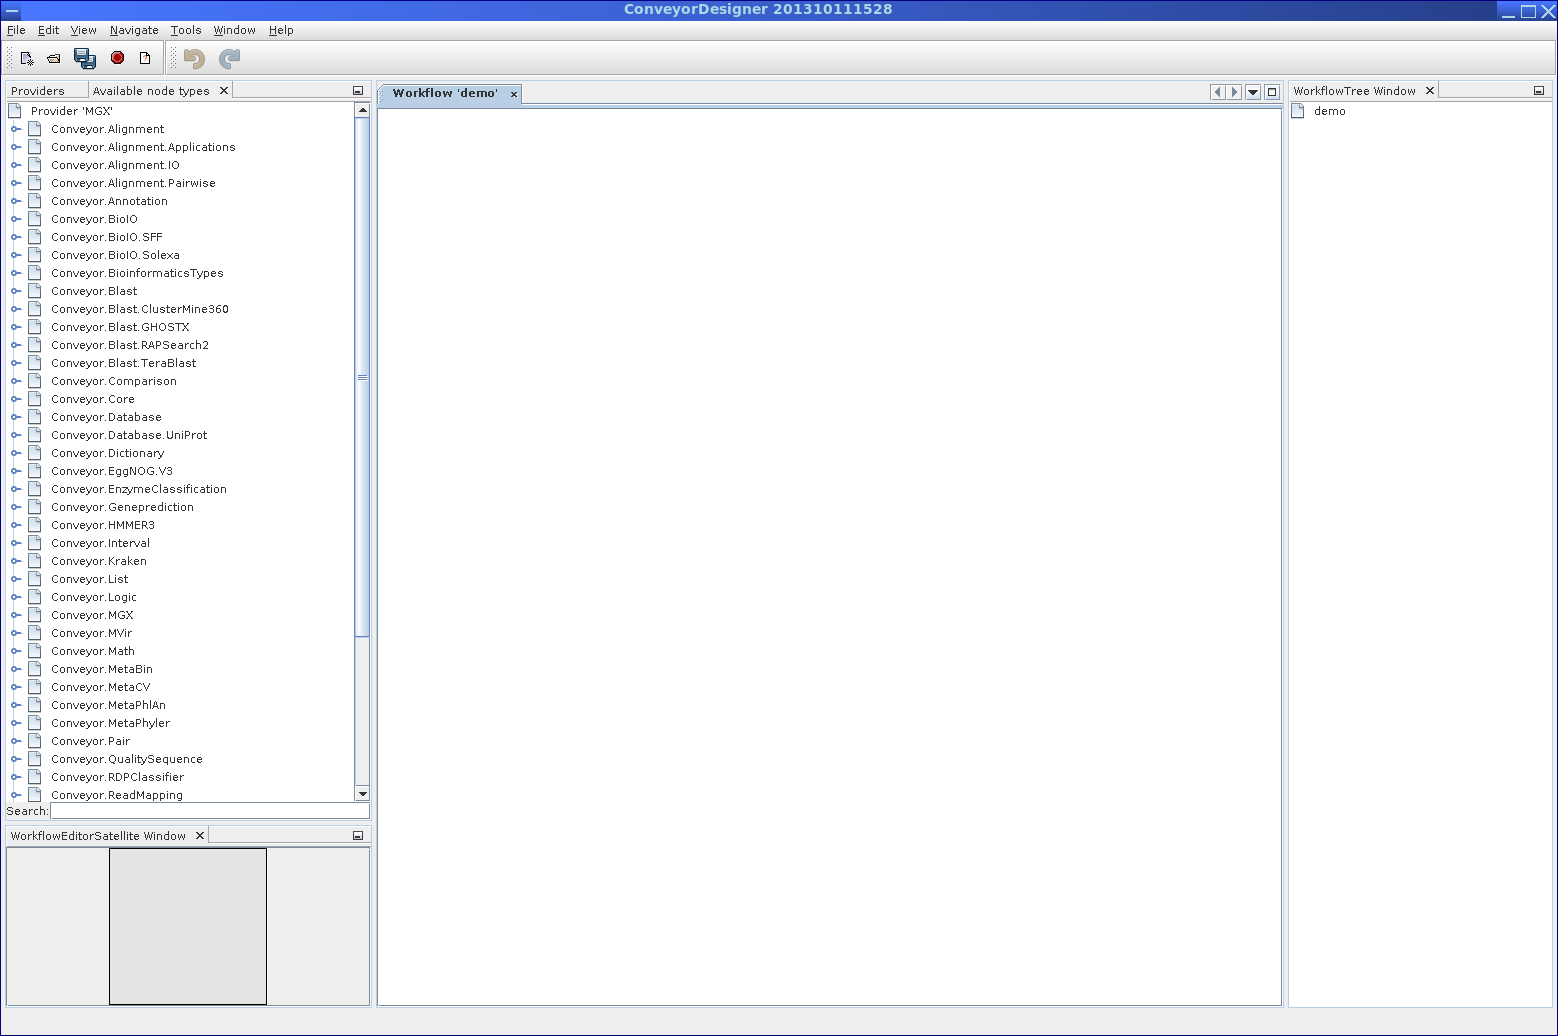
\includegraphics[width=\textwidth]{img/conveyor/designer}
\caption[Conveyor Designer]{The Conveyor Designer application allows easy and user-friendly
development of custom analysis algorithms in a graphical way.}
\label{designer}
\end{figure}

As Conveyor is actively developed and new tools are continously integrated, giving a thorough
introduction to Conveyor is beyond the scope of this document. The most up-to-date documentation describing
Conveyor itself and the Conveyor Designer in particular can be found at the Conveyor web
site \url{http://www.uni-giessen.de/fbz/fb08/bioinformatik/software/Conveyor}. 

\section{Getting started}

In order to implement a custom workflow, the Conveyor Designer needs to be configured
with a definition of available Conveyor plugins and node types. This is easily 
achieved by importing a plugin dump file, which contains a list of data types and
nodes provided by a Conveyor installation.

To use the Designer to implement a workflow for the MGX framework, a corresponding
plugin dump file can be obtained from within MGX by right-clicking on the 
project name (\ref{getdump}).

\begin{figure}[H]
\centering
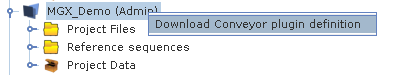
\includegraphics[width=.5\textwidth]{img/conveyor/getdump}
\caption[Plugin dump.]{A plugin dump file for use with the Conveyor Designer can be obtained from within MGX
by right-clicking on the project name.}
\label{getdump}
\end{figure}

Afterwards, start the Designer application and define a new provider (Right-click on ``Available providers''). 
Make sure to specify ``Plugin dump file'' (\ref{loaddump}) as the type of plugin set and select the file
generated by MGX. Once the plugin
dump file has been imported, you are ready to implement new workflows. Initially starting with an empty sheet,
nodes can be dragged from the list of all available nodes on the left and placed onto the sheet. Node connections
are created by clicking on a node, keeping the mouse button pressed and releasing it over the connections target
node, thus creating the link; in ambiguous cases, e.g. for nodes with several unconnected
inputs/outputs, a dialog will allow to select the desired connection.
Nodes may also require node-specific configuration, which can be edited from a nodes context menu.
A red border around a node indicates missing configuration items or connections.

\begin{figure}[H]
\centering
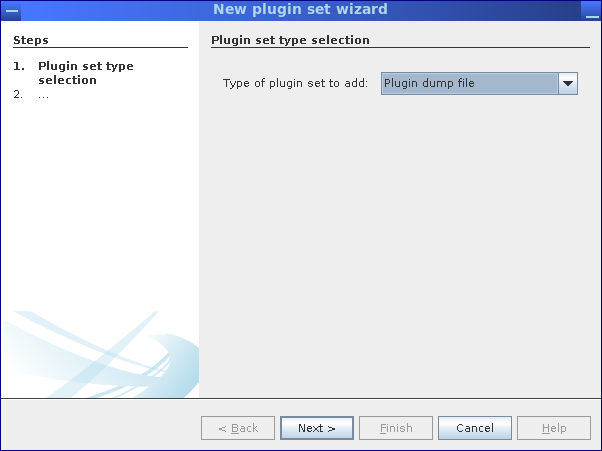
\includegraphics[width=.7\textwidth]{img/conveyor/loaddump}
\caption[Adding a new provider.]{Importing a plugin dump file into the Conveyor Designer.}
\label{loaddump}
\end{figure}

\section{Workflow requirements}

In order to design custom Conveyor workflows for later usage within the MGX platform, there
are several constraints to be met which will be described in more detail.\\

First of all, a dedicated \node{GetMGXJob} node (Figure \ref{getmgxjob}) has to be present within the workflow; in addition,
this node has to be named "\textbf{mgx}". During execution of a pipeline within MGX, this node is
configured via an external configuration file, providing required information about a jobs
context, like e.g. access to a project database and associated storage.\\

\begin{figure}[H]
\centering
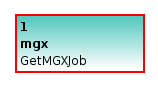
\includegraphics[width=.3\textwidth]{img/conveyor/getjob}
\caption[\node{GetMGXJob}]{The \node{GetMGXJob} node provides necessary context for executing a
workflow within MGX, such as database access. By convention, this node has to be named \textbf{mgx}.}
\label{getmgxjob}
\end{figure}

Access to metagenome DNA sequences is provided via the \node{ReadCSF} node, which will provide
all metagenome sequences for a sequencing run object within MGX, except those for which the 
``discard'' flag has already been set. As pipelines are always executed
for one single analysis job, this node needs to be connected to the \node{GetMGXJob} node (\ref{readcsf}).
Figure \ref{simple} shows a minimal example of a Conveyor-based pipeline for use within the MGX framework.
Once executed, the pipeline would set the \textit{discard} flag for all sequences.

\begin{figure}[H]
\centering
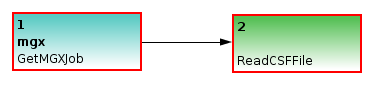
\includegraphics[width=.6\textwidth]{img/conveyor/getjobreadcsf}
\caption[\node{ReadCSF}]{The \node{ReadCSF} node is used to obtained metagenome sequence data 
from within MGX; it has one input and needs to be connected to the \node{GetMGXJob} node.}
\label{readcsf}
\end{figure}

\begin{figure}[H]
\centering
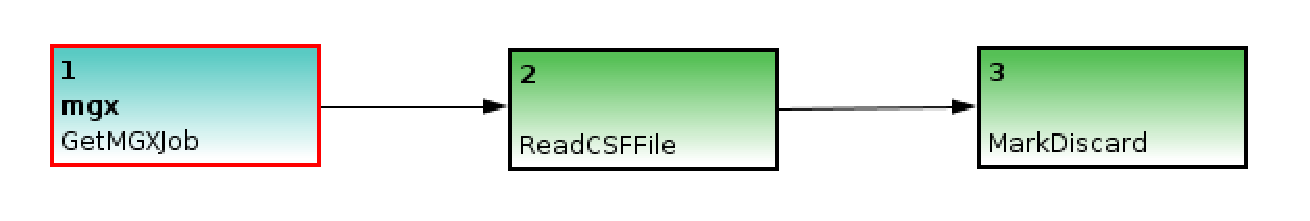
\includegraphics[width=.8\textwidth]{img/conveyor/simple}
\caption[Minimal example]{A minimal working example of a pipeline developed for MGX, which would set the \textit{discard} flag for all sequences.}
\label{simple}
\end{figure}


\section{Annotating metagenome sequences}

\begin{figure}[H]
\centering
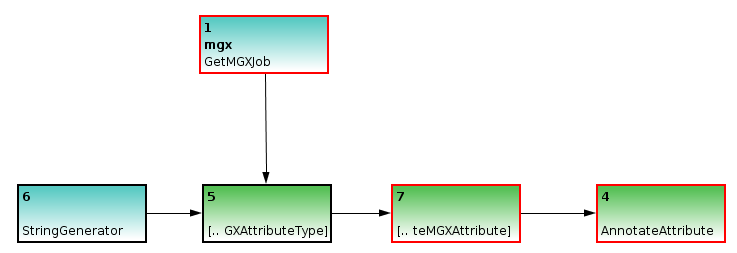
\includegraphics[width=.85\textwidth]{img/conveyor/annotate_templ}
\caption[Metagenome annotation]{Basic template to illustrate sequence annotation. A \node{StringGenerator} is
used to generate a label for the attribute type (\node{CreateMGXAttributeType}), which also requires job context
information. The attribute type is required to create attributes, thus the node is connected to the \node{CreateMGXAttribute} node. Finally, the annotation can be saved to the project database (\node{AnnotateAttribute} node).}
\label{annot}
\end{figure}

Annotation of metagenome sequences requires an ``attribute type'' and an ``attribute''. As an example, we will
illustrate the implementation of a pipeline for the analysis of GC content within metagenome sequences.
We use a \node{StringGenerator} node configured to generate the string ``GC'' to create a label for the
attribute type. As GC content is indicated by a number, we appropriately configure the \node{CreateMGXAttributeType}
node to emit a \textbf{basic} (i.e. not hierarchical) as well as numerical ``attribute type'' (\ref{createattrtype}).

\begin{figure}[H]
\centering
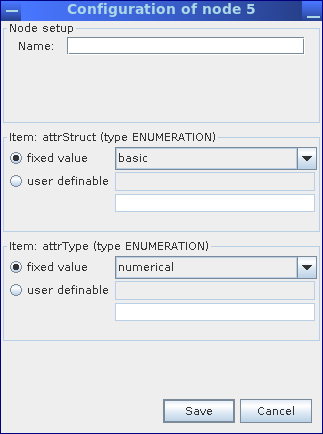
\includegraphics[width=.5\textwidth]{img/conveyor/createattrtype}
\caption[Defining an attribute type.]{Within the configuration dialog for the \node{CreateMGXAttributeType} node, structure and type of the generated attribute values are defined.}
\label{createattrtype}
\end{figure}

\begin{figure}[H]
\centering
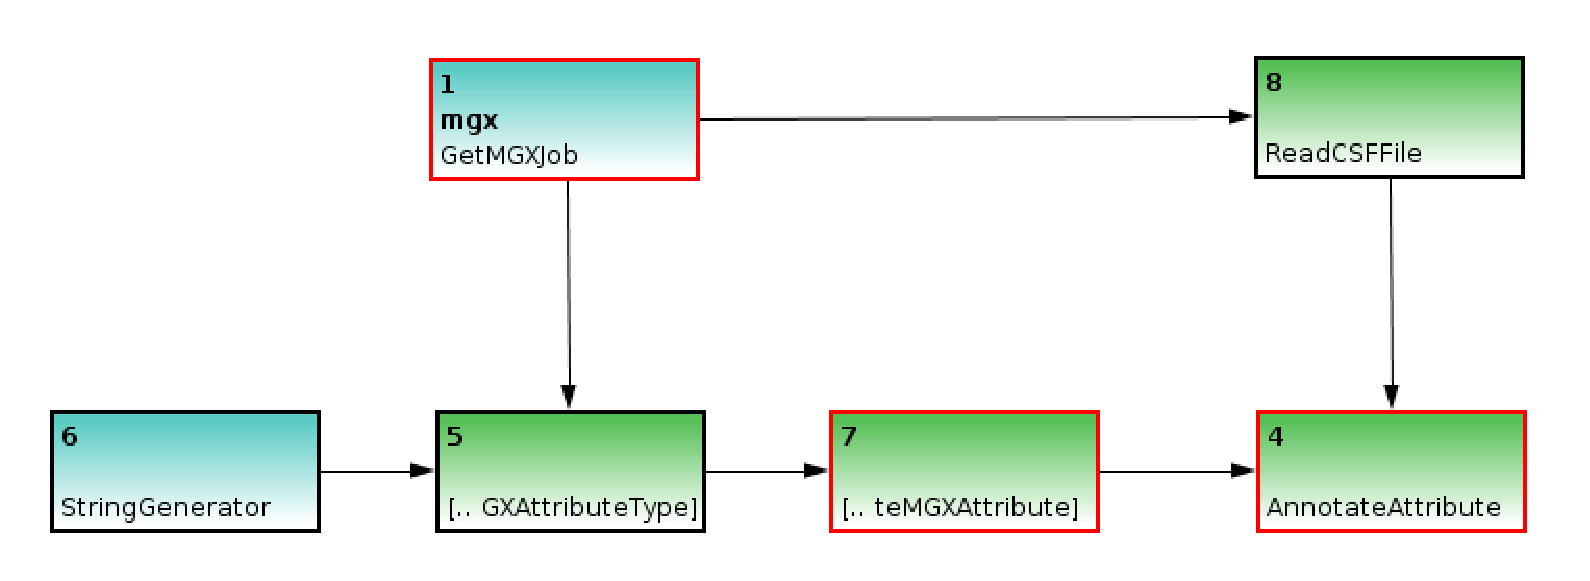
\includegraphics[width=.8\textwidth]{img/conveyor/annotate_templ2}
\caption[Metagenome annotation]{Incomplete example; extending upon \ref{annot}, the \node{ReadCSF} node will
provide the necessary metagenome sequences to be annotated. Still, there is no actual analysis specified.}
\label{annot2}
\end{figure}

In a second step, we use the \node{ReadCSF} node to obtain access to the individual metagenome sequences; as 
MGX annotates sequences individually, a connection between \node{ReadCSF} and \node{AnnotateAttribute} is
required (\ref{annot2}). Subsequently, we implement the actual analysis, which is provided by the \node{GCContent}
node. It will process all sequences sequentially and the GC content will be used to create a corresponding
attribute (\ref{annot3}).

\begin{figure}[H]
\centering
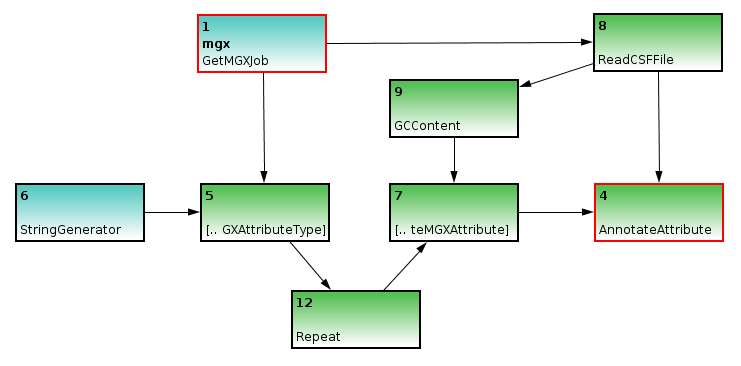
\includegraphics[width=.8\textwidth]{img/conveyor/annotate_templ3}
\caption[Metagenome annotation]{Step 2: The \node{GCContent} node represents the actual analysis step; it is used
to determine the GC content of a DNA sequence, which will then be converted into an ``attribute''.}
\label{annot3}
\end{figure}

Finally, as an annotation always refers to only a part of a sequence, we will need to generate the corresponding
start and end coordinates; since GC content refers to the full sequence, we can use an \node{ULongGenerator} node
configured to emit 0 (MGX uses 0-based coordinates) to generate the start coordinate; the end coordinate can be
created based on the sequences' length, obtained through the \node{GetLength} node (\ref{annot4}).\\
The \node{GetMGXJob} node will retain its red border due to missing configuration; this, however, can be
ignored, as appropriate configuration will be provided by the MGX framework automatically.

\begin{figure}[H]
\centering
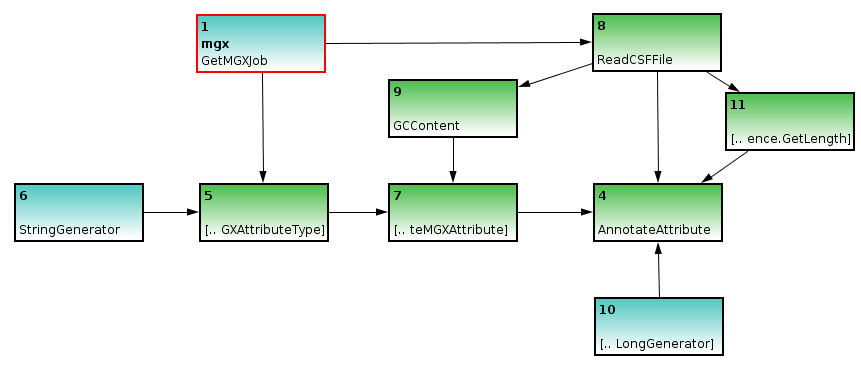
\includegraphics[width=.9\textwidth]{img/conveyor/annotate_templ4}
\caption[Metagenome annotation]{Completing the workflow: the \node{ULongGenerator} and \node{GetLength} nodes
are added to specify coordinates for the subregion of the DNA sequence described by the ``attribute''.}
\label{annot4}
\end{figure}

\subsection{Creating hierarchical attributes}

Annotation of hierarchical attributes requires a little more effort. The \node{CreateHierarchicalMGXAttribute} node
is used to obtain the inner structure of the hierarchy in a bottom-up approach; It contains several loops which
will be explained in more detail.

\begin{figure}[H]
\centering
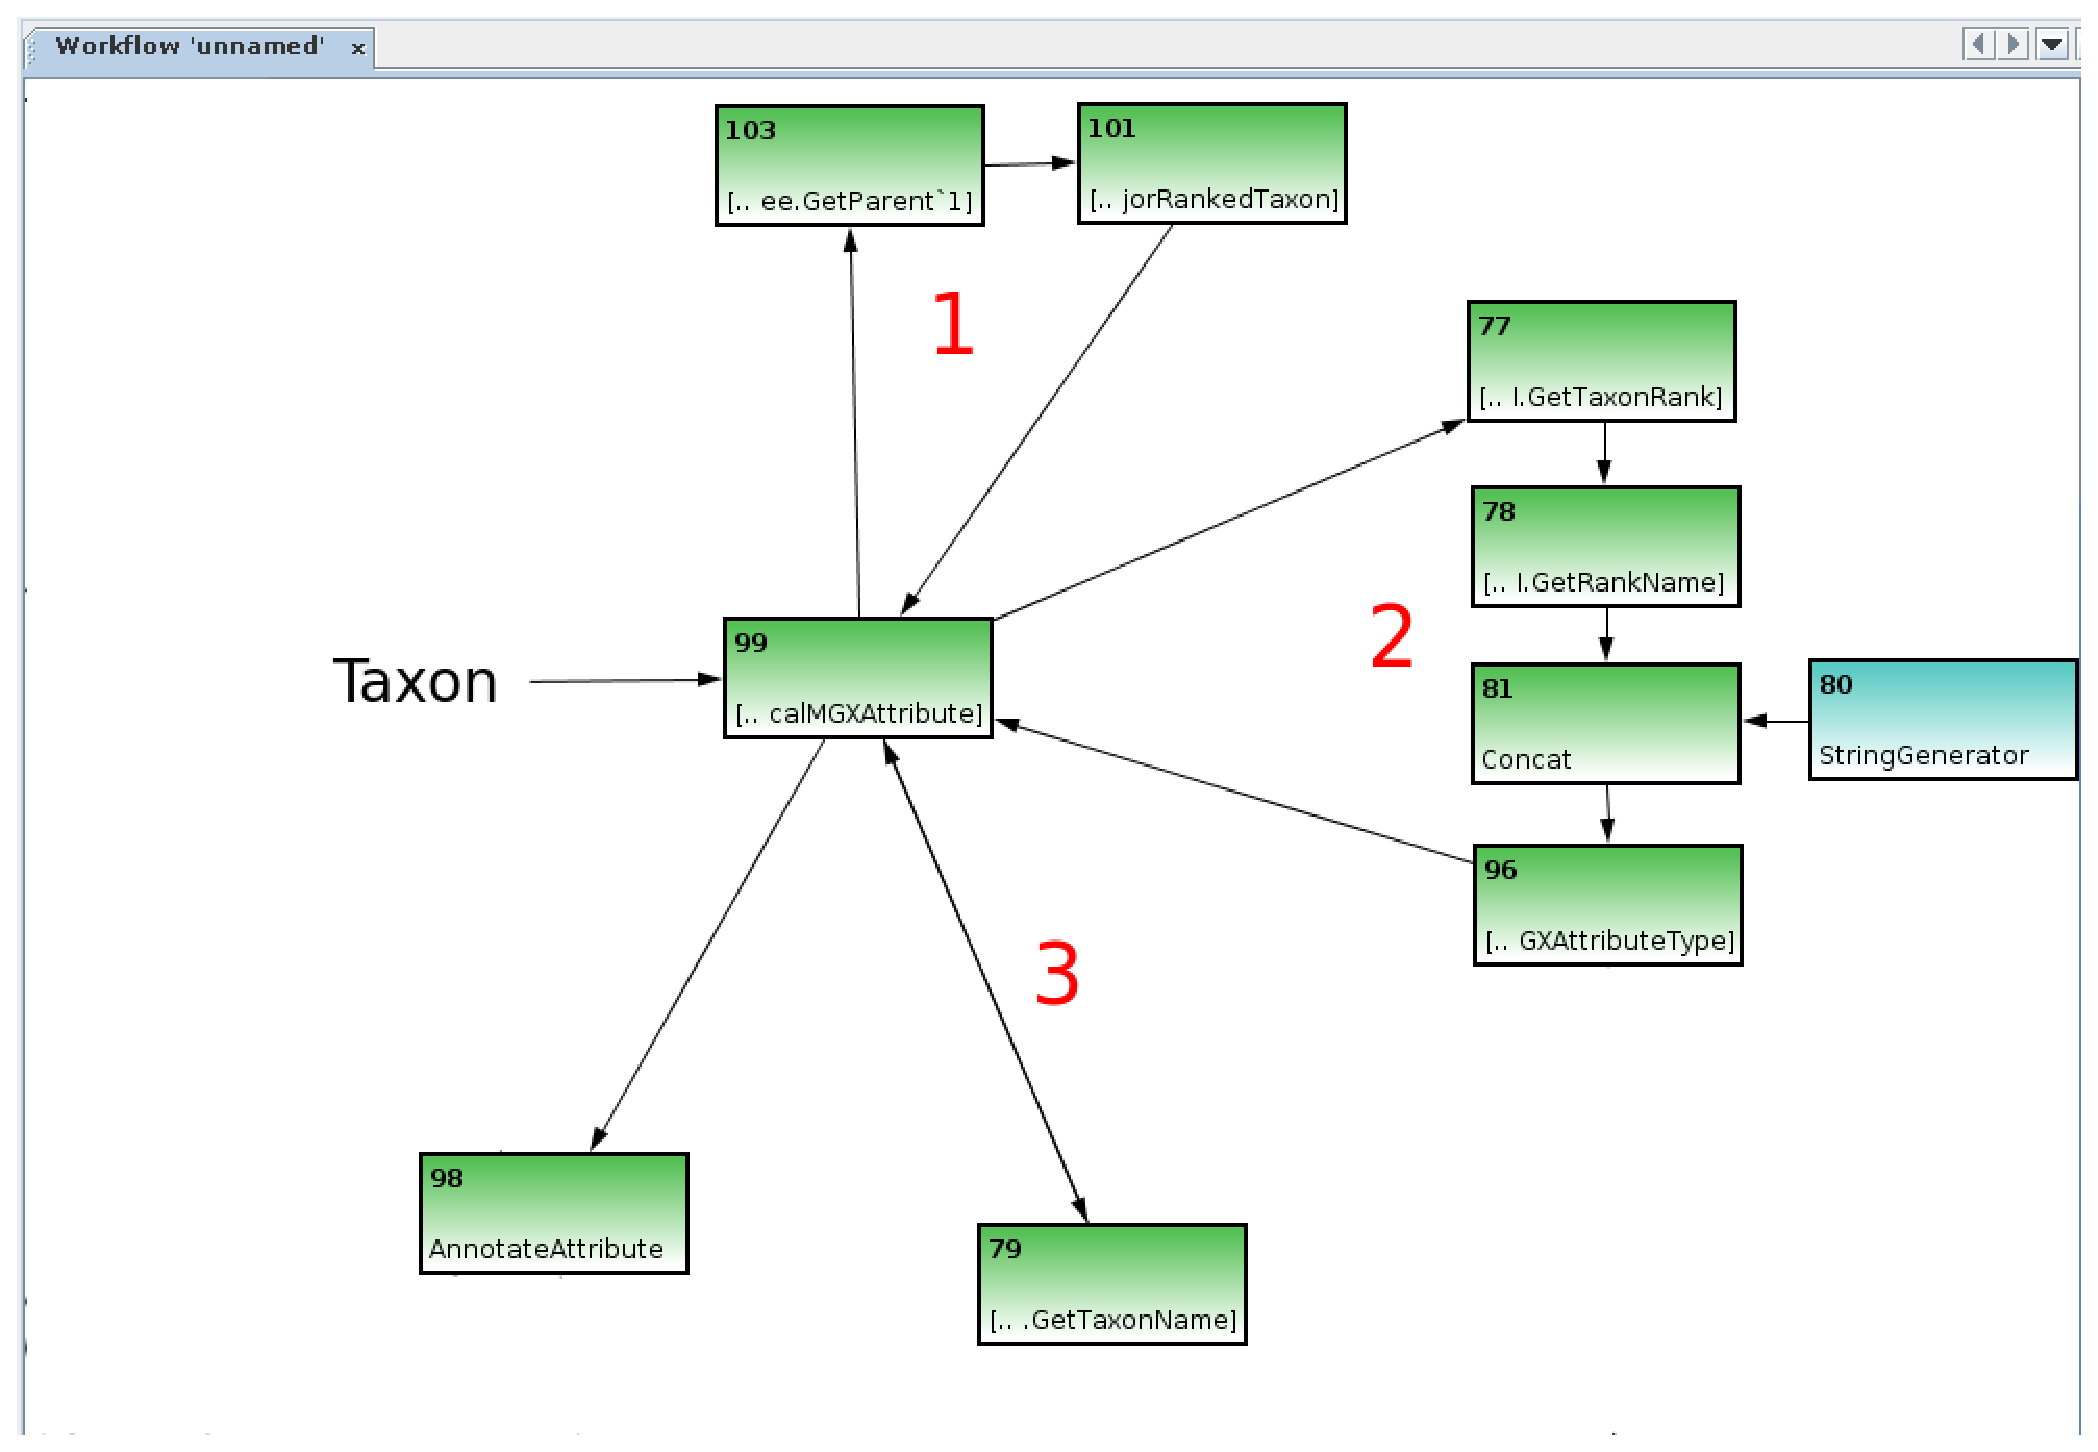
\includegraphics[width=\textwidth]{img/conveyor/TreeAnnot}
\caption[Hierarchical attributes]{The \node{CreateHierarchicalMGXAttribute} node required three loops
to create the internal structure of the hierarchy. Several connections were removed from the figure
for illustrative purposes.}
\label{annot5}
\end{figure}

A single object, e.g. a NCBI taxon generated by the Kraken\cite{KRAKEN} classifier, is provided as an input
into the node (\ref{annot5}). 
The first loop is required to obtain the objects parent object, thus defining the hierarchy. In this example
it is implemented using the \texttt{GetParent} and \texttt{GetMajorRankedTaxon} nodes, thus making sure only
the major taxonomic ranks (superkingdom, phylum, class, \dots) are included.\\
The second loop is used to obtain the corresponding attribute type for the parent: it operates on the parent
object obtained by the first loop. \texttt{GetTaxonRank} and \texttt{GetRankName} nodes provide the corresponding
ranks' name, e.g. ``class''; The \texttt{StringGenerator} and \texttt{Concat} nodes are then used to create the
attribute type: ``NCBI\_class''. This value is used to create the corresponding attribute type employing the
\node{CreateMGXAttributeType} node, which is returned into the \node{CreateHierarchicalMGXAttribute} node.\\
The third and final loop is used to map a data object to its name, which is used to create the attributes value;
it is built up using the \texttt{GetTaxonName} node, which delivers its output back into the node.\\

Thus, the three loops might be termed as \textbf{Get parent}, \textbf{Get AttributeType for object} and
\textbf{Generate value}. 

The \node{CreateHierarchicalMGXAttribute} node emits an initial MGXAttribute for the incoming data object,
with the corresponding AttributeType provided by loop 2 and the MGXAttribute's value obtained using loop 3.
Subsequently, loop 1 is used repetitively until the root node is reached, with all intermediary results
passing through loops 2 and 3, thus generating a single path of hierarchical attributes within the taxonomic
tree. The output of the \node{CreateHierarchicalMGXAttribute} is connected to the \node{AnnotateAttribute}
node as in the previous example.

For brevity's sake, several connections are hidden within the image, which have already been explained in the
previous section; the \node{CreateMGXAttributeType} node needs an incoming connection providing a MGXJob,
and the \node{AnnotateAttribute} node requires additional connections providing the sequence to be annotated
and start/stop coordinates for the subregion which is described by the annotation.




%
\chapter{Advanced usage: Extending the MGX platform}
\label{extending}

\section{Implementing new visualizations}

Tree\\
Distribution\\
ViewerI\\



%\chapter{Literatur}

\bibliographystyle{apalike}
%\bibliography{literatur}
%\bibliographystyle{da}
\bibliography{ref}

\listoffigures
\listoftables

% -----------------------------------------------------------
%\backmatter
\begin{appendix}

\end{appendix}

\end{document}
